%\documentstyle[rotate,page,epsf,epsfig,url,subfigure,wrapfig,floatflt]{article}
% Switching to Latex2e instead of 2.09
\documentclass[10pt]{article}
\usepackage{rotate,page,epsf,epsfig,url,subfigure,wrapfig,floatflt,algorithm2e}
\usepackage[sc]{mathpazo}
\usepackage{amsmath}
\usepackage{epstopdf}
%\usepackage{verse}

% Using 10.5 fonts over 11pt skips. (Actual lines/inch is achieved also with
% the linespread above
%\renewcommand{\normalsize}{\fontsize{10.5pt}{11pt}\selectfont}

% removed times -- since apparently not allowed by NSF
%\newcounter{definition}
\newtheorem{theorem}{Theorem}
\newtheorem{axiom}[theorem]{Axiom}
\newtheorem{case}[theorem]{Case}
\newtheorem{claim}[theorem]{Claim}
\newtheorem{conclusion}[theorem]{Conclusion}
\newtheorem{conjecture}[theorem]{Conjecture}
\newtheorem{corollary}{Corollary}
\newtheorem{definition}{Definition}
\newtheorem{example}{Example}
\newtheorem{lemma}{Lemma}
\newtheorem{proposition}[theorem]{Proposition}
\newtheorem{remark}[theorem]{Remark}
%\def\proof{\noindent\hspace{2em}{\it Proof: }}

\newcommand{\Geotags}{GLUE}

\newcommand{\aiaaJGCD}{AIAA Journal of Guidance, Control and Dynamics}
\newcommand{\ieeeTCST}{IEEE Transactions on Control Systems Technology}
\newcommand{\ieeeTITS}{IEEE Transactions on on Intelligent Transportation Systems}
\newcommand{\ieeeTAC}{IEEE Transactions on Automatic Control}
\newcommand{\TransResB}{Transportation Research - B}
\newcommand{\ieeeCSM}{IEEE Control Systems Magazine}
\newcommand{\JCP}{Journal of Computational Physics}
\newcommand{\JFM}{Journal of Fluid Mechanics}
\newcommand{\ECC}{Proceedings of the European Control Conference}
\newcommand{\ACCotwo}{American Control Conference}
\newcommand{\ACCofour}{American Control Conference}
\newcommand{\CDCothree}{Proceedings of the $42^{\text{nd}}$ IEEE Conference on Decision and Control}
\newcommand{\CDCnintyfive}{Proceedings of the $34^{\text{th}}$ IEEE Conference on Decision and Control}
\newcommand{\ESAIM}{ESAIM: {C}ontrol, {O}ptimisation and{C}alculus of {V}ariations}
\newcommand{\SysContLet}{Systems \& Control Letters}
\newcommand{\SIAMJCO}{SIAM Journal of Control Optimization}
\newcommand{\procRSLsAMPS}{Proceedings of the Royal Society of London. Series A, Mathematical and Physical Sciences}
\newcommand{\systemname}{{\em Headbanger}}
\newenvironment{itemizer}{\begin{itemize}\setlength{\parsep}{0cm}\setlength{\itemsep}{-.3em}}{\end{itemize}}
\newenvironment{enumerator}{\begin{enumerate}\setlength{\itemsep}{-0.15cm}}{\end{enumerate}}

\newcommand{\argmax}{\operatornamewithlimits{argmax}}

\newif\ifremark
\long\def\remark#1{
\ifremark%
	\begingroup%
	\dimen0=\columnwidth
	\advance\dimen0 by -0.25in%
	\setbox0=\hbox{\parbox[b]{\dimen0}{\protect\em #1}}
	\dimen1=\ht0\advance\dimen1 by 2pt%
	\dimen2=\dp0\advance\dimen2 by 2pt%
	\vskip 0.25pt%
	\hbox to \columnwidth{%
		\vrule height\dimen1 width 3pt depth\dimen2%
		\hss\copy0\hss%
		\vrule height\dimen1 width 3pt depth\dimen2%
	}%
	\endgroup%
\fi}

\remarkfalse

\usepackage{vmargin}
\setpapersize{USletter}
\setmarginsrb{0.9in}{0.8in}{.9in}{.9in}%
{0in}{0in}{0in}{0.0in}

\linespread{1.029} %% use this to control line spacing

\begin{document}



\setcounter{page}{1}
\def\mysection{A}
\nsffoot \nsftitle{Project Summary}

\begin{center}
\vspace{-6mm}
{\bf TWC: Small: Authenticating Smart Wearable Devices Using Unique Human Body Movement Patterns\\ Zhang, Rutgers University\\}
\end{center}
\vspace*{-2mm}

\input{hb_summary}

%\vspace*{-1mm}
%\begin{center}
%\begin{tabular*}{\textwidth}{l@{\extracolsep{\fill}}r}
%Yanyong Zhang, Wade Trappe, Richard Howard  & {\bf WINLAB, Rutgers University}\\
%\end{tabular*}
%\end{center}
%%\vspace*{.1in}
\pagebreak




\setcounter{page}{1}
\def\mysection{C}
\nsffoot \nsftitle{PROJECT DESCRIPTION}
\def\thesection{\arabic{section}}
\def\thesubsection{\arabic{section}.\arabic{subsection}}
\def\thesubsubsection{\arabic{section}.\arabic{subsection}.\arabic{subsubsection}}
%\remark{
%}
\section{Introduction}\label{sec:intro}
After generations of technological revolutions, from wired to wireless communications, stationary to mobile machines, and large-sized to hand-held devices, we are now witnessing what can be deemed as the
next phase of mobile technology: widespread {\em wearable computers}. Research in
wearable computers can be dated back at least to the 1980s when Steve Mann
experimented with backpack computers and developed a prototype of heads-up-display goggles~\cite{mann1997wearable}. Thanks to the advances in hardware miniaturization technology, cheap sensors/processor
chips, and low-power sensing/computing, today, wearables are now available
off-the-shelf and on the way to become an integral part of human
lives~\cite{googleglass,smartwatch,fitbit}. In this proposal, we focus in this proposal, we focus on special-purpose wearable devices that are worn close to the body as opposed to the more general-purpose computing/communication platform like smartphones or tablets. Examples are smart glasses, smart wristbands, and smart watches, smart jewelry, and devices embedded in clothing like jackets or shoes. Such devices are typically very small and impose severe resource constraints.

With the proliferation of such wearable devices, they can be expected to be subjected to malicious attacks and preserving the security and privacy of these devices will become increasingly important.
Much of the collected data on such devices is personal in nature and often relates to the user's health. Any security and privacy solution for such devices, however, also has to strike an appropriate balance with user convenience, especially as users are interacting with an increasing number of such specialized devices. A fundamental building block for safeguarding the security and privacy of user data acquired on or accessed through wearable devices are user authentication techniques, since many solutions are only effective as long as the device itself is authenticated to the right user/owner.

Authentication on most commercially available wearable devices today~\cite{fitbit, smartwatch} relies on an indirect mechanism, where users can log in to their wearables through their phones. This requires the wearable device to be registered and paired to the user's mobile device, which makes it inconvenient as the user has to carry both devices. The security of this approach is also in question as it increases the chance of hacking into both the devices if either of the devices are lost or stolen. Some devices including Google Glass~\cite{googleglass} and FitBit's health tracker~\cite{fitbit} also allow linking the device to online accounts instead of the phone for user's convenience; however, this does not add any security benefit. Indirect authentication remains a dominant paradigm for wearables despite these fundamental shortcomings because these devices are \emph{seriously resource-constrained} in many aspects: battery power, computational and storage capabilities, and input/output methods. As a result, typical authentication methods designed for more powerful devices can not be directly applied and must operate indirectly through a paired smartphone or other more capable device. In this proposal, however, we take the viewpoint that wearables will become more independent units that have to maintain security guarantees without such paired devices and we seek to develop suitable \emph{direct authentication} methods that are both accurate and light-weight.

Before we design direct authentication methods for wearable devices, let us first consider the available solutions for other mobile systems, especially smartphones and tablets. Broadly speaking, the two most commonly used authentication methods on mobile systems are arguable password-based methods (with their variants) and biometric-based methods. However, we argue that neither of these two methods is really suitable for wearable devices. Typing passwords or drawing swipe patterns on wearable devices can be quite cumbersome due to their small input/output units, if they do have a touch sensor at all. Collecting and recognizing physiological biometrics (such as DNA, fingerprint, hand/finger geometry, iris, odor, palm-print, retinal scan, voice, etc.) requires specialized sensing hardware and processing resources that add cost, and many of these sensors are larger than the size of wearables themselves.

This project therefore focuses on a third class of direct authentication methods: relying upon the uniqueness of human behavior characteristics such as human walking gait, arm swings, typing patterns, body pulse beats, eye-blinks, etc. This way of authenticating users is often referred to as \emph{behavioral} biometrics, and existing work has largely studied it in the context of authenticating smart phones and tablets~\cite{rahman2014bodybeat,cornelius2014wearable,stevenage1999visual,okumura2006study,monrose2000keystroke,jorgensen2011mouse,bo2013silentsense,de2012touch}. The main advantage of using behavioral biometrics for mobile devices is that the signatures can be readily generated from raw data of built-in sensors such as motion sensors, camera, microphones etc. Considering that cameras and microphones, as well as vision/audio processing algorithms, are quite energy-hungry, we thus focus on those behavioral biometrics that can be easily captured by sensors that require less power consumption, such as accelerometer and gyroscope. More specifically, we propose to authenticate wearable devices to users based on one type of behavioral characteristics: our unique body movement patterns and their dependence on external stimuli that wearable devices can generate, such as vibrations and music.

Body movement patterns have long been used by us humans to discriminate between people. By watching how a person walks, dances, waves her hands, we can often recognize the person from afar. This is because human body movements are \emph{distinctive} and \emph{repeatable}.  Achieving the same through wearables, however, is not straightforward and poses significant research challenges: it is unclear whether these seriously-constrained devices are able to capture the movement patterns, process the data, and quantify the uniqueness of each user's behaviors. Moreover, each device will have only a limited view of body movements, dependent on its mounting position on the human body. In this proposal, we set out to conduct a holistic study of wearable authentication through body movements and to design an accurate, robust and light-weight authentication system. A key distinguishing feature of our work is that we will also consider stimuli that wearable devices can provide to design challenge-response inspired mechanisms, particularly stimuli that are difficult to observe even for the closest adversaries. For example, we can use fast-tempo music through earbuds to stimulate movements and to make such free-style movements more repeatable. Our preliminary investigations show that under very controlled experiments, music-stimulated body movements have great potential to be used to authenticate users to their wearable devices. In order to develop a full-fledge authentication system that works in realistic settings, we propose several techniques to maximize the authentication accuracy and robustness by trying to increase the information encoded in sensor signals, exploiting multiple movements and/or multiple sensors, learning how to authenticate users in mobile settings, and designing movement pattern-based ``passwords'', as well as minimize its power consumption and processing requirement by carefully selecting features and classifiers, pipelining authentication operations and dynamically adjusting the data sampling rate. We will consider features of movements pattern that are more biometric in nature as well as those that depend more on user knowledge. For example, a list of motions associated with different prompts/stimuli can take the place of a 'password'.

Our research involves a coordination of algorithm design and system evaluation, ultimately involving the construction of a realistic authentication system that can efficiently run on wearable devices. Our project also involves an important curriculum development effort. We intend to train next-generation workforces in the rapidly-growing wearable and mobile computing field, as well as recruit youth and women into research in this field.



\section{Background and Overview} \label{sec:background} 
\begin{figure*}[t]
\begin{center}
\begin{tabular}{ccc}
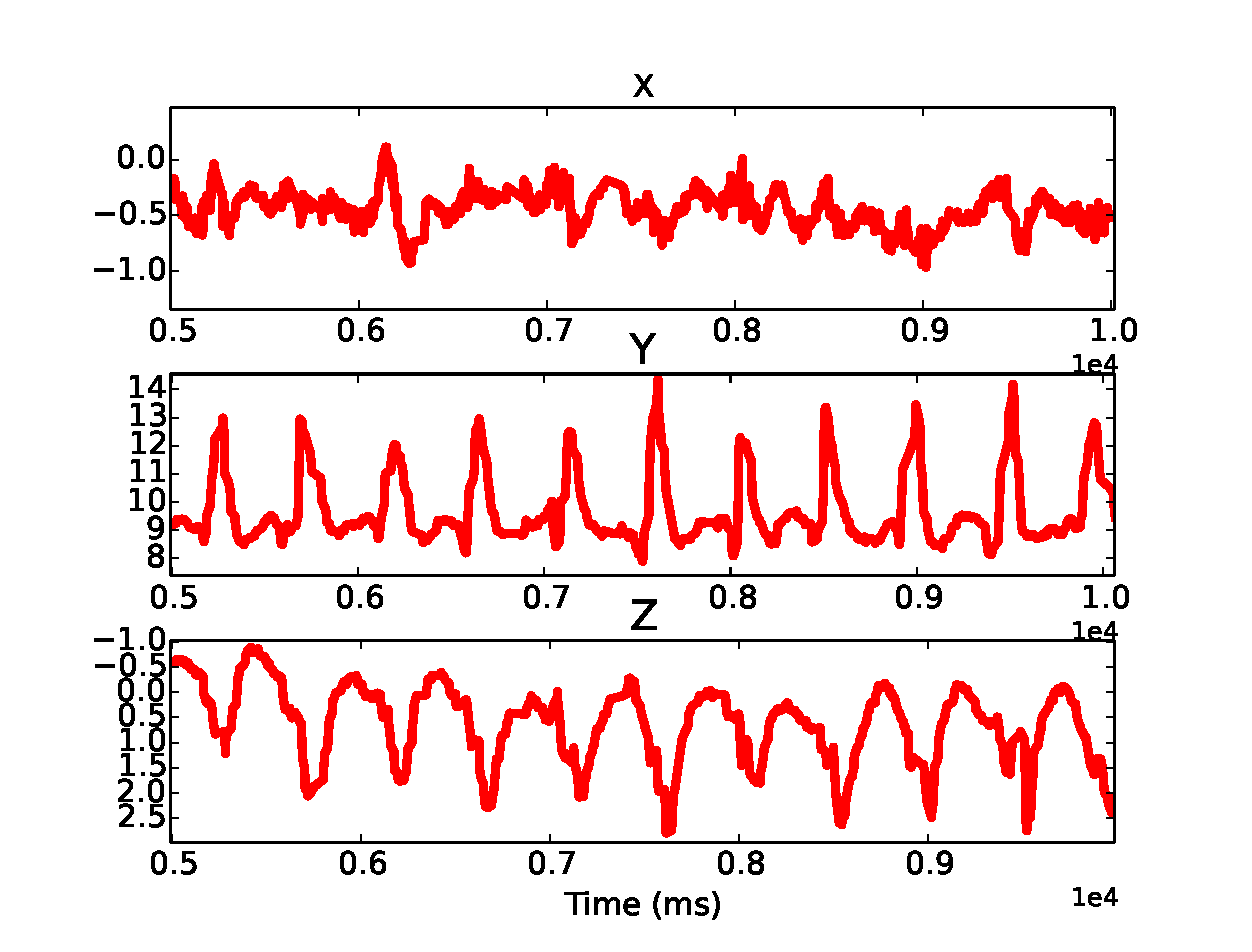
\includegraphics [width=.33\linewidth]{../mobisys_paper/fig/raw_sub1.eps}&
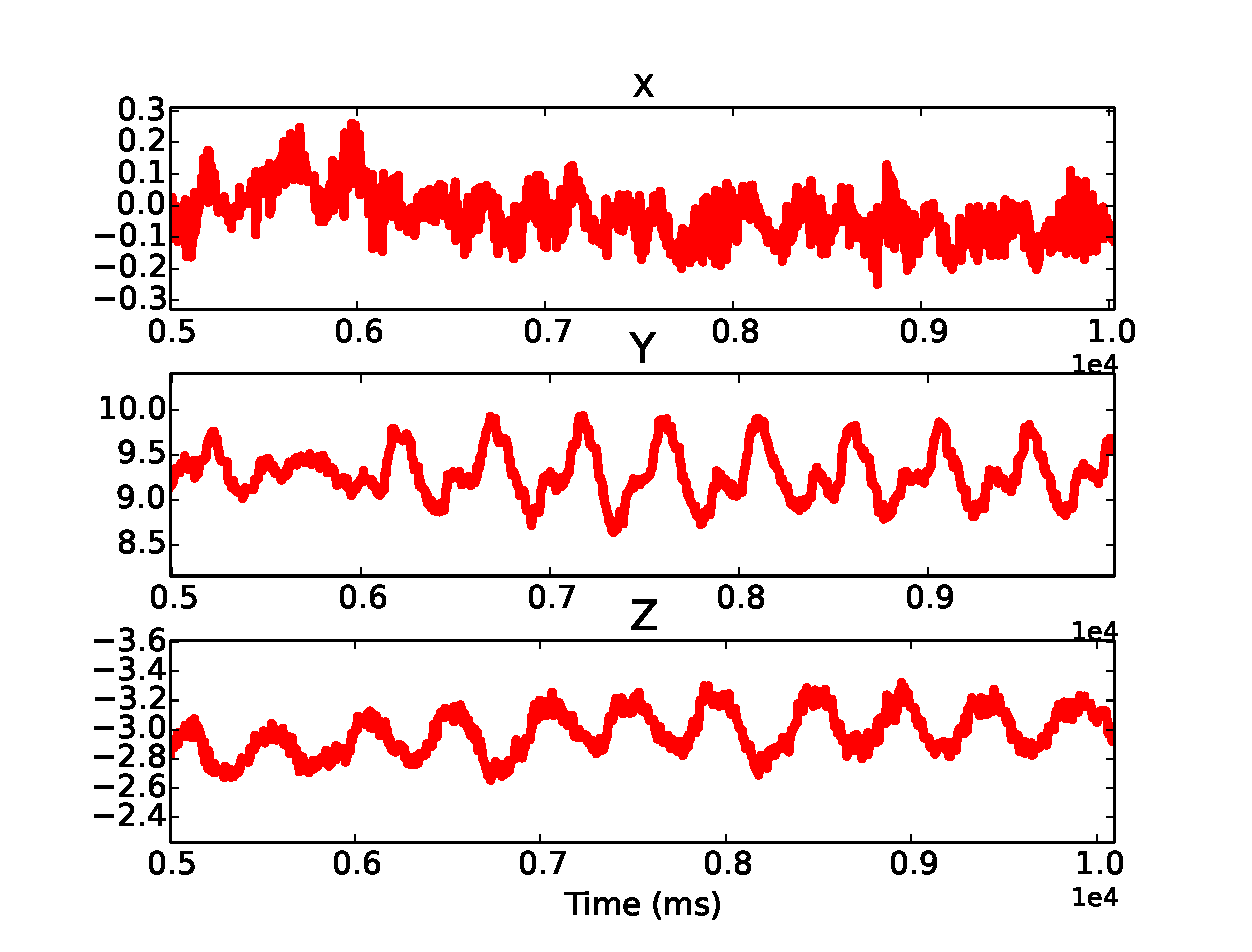
\includegraphics [width=.33\linewidth]{../mobisys_paper/fig/raw_sub8.eps}&
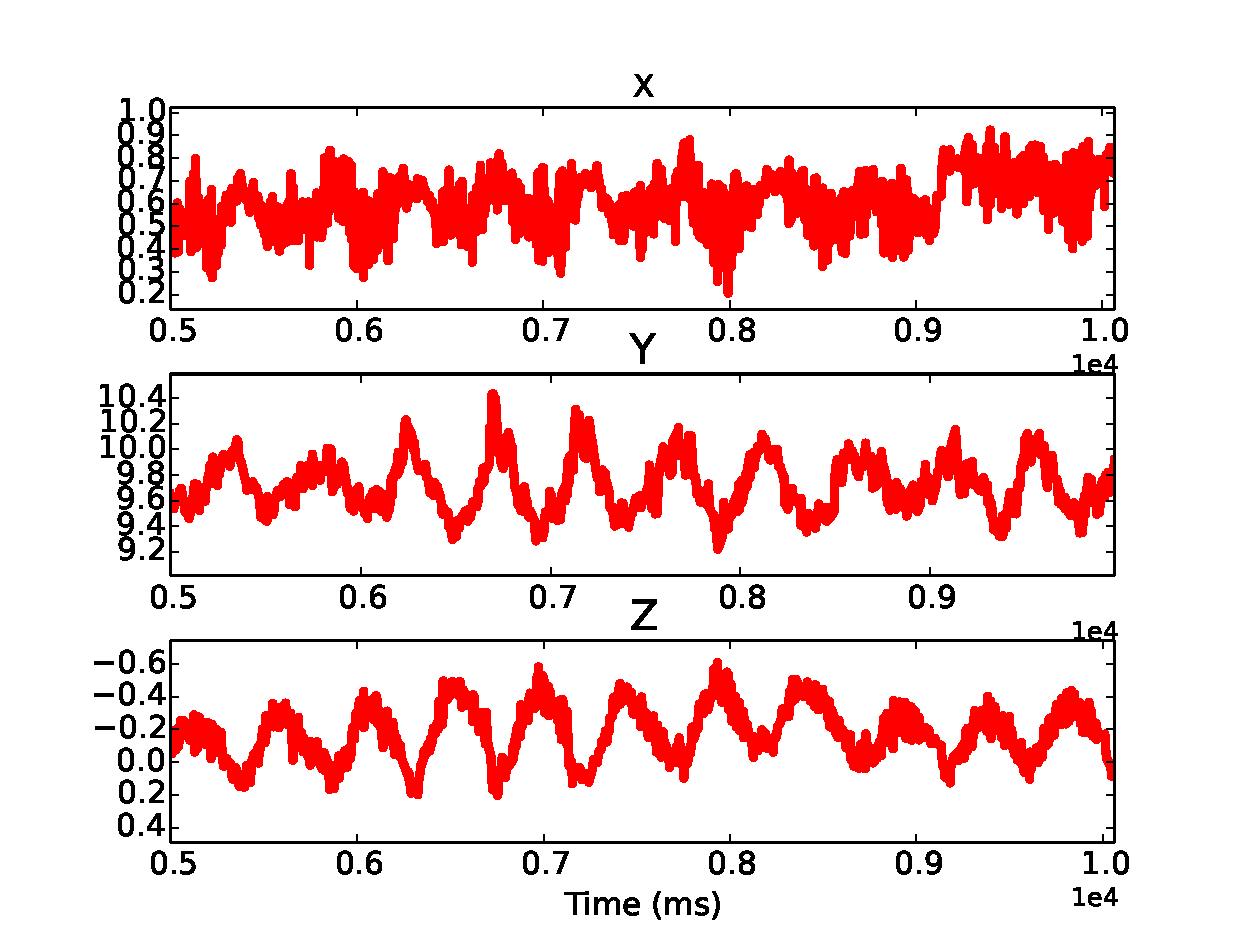
\includegraphics [width=.33\linewidth]{../mobisys_paper/fig/raw_sub3.eps}\\
(a) User 1& (b) User 2 & (c) User 3 \\
\end{tabular}

\begin{tabular}{cc}
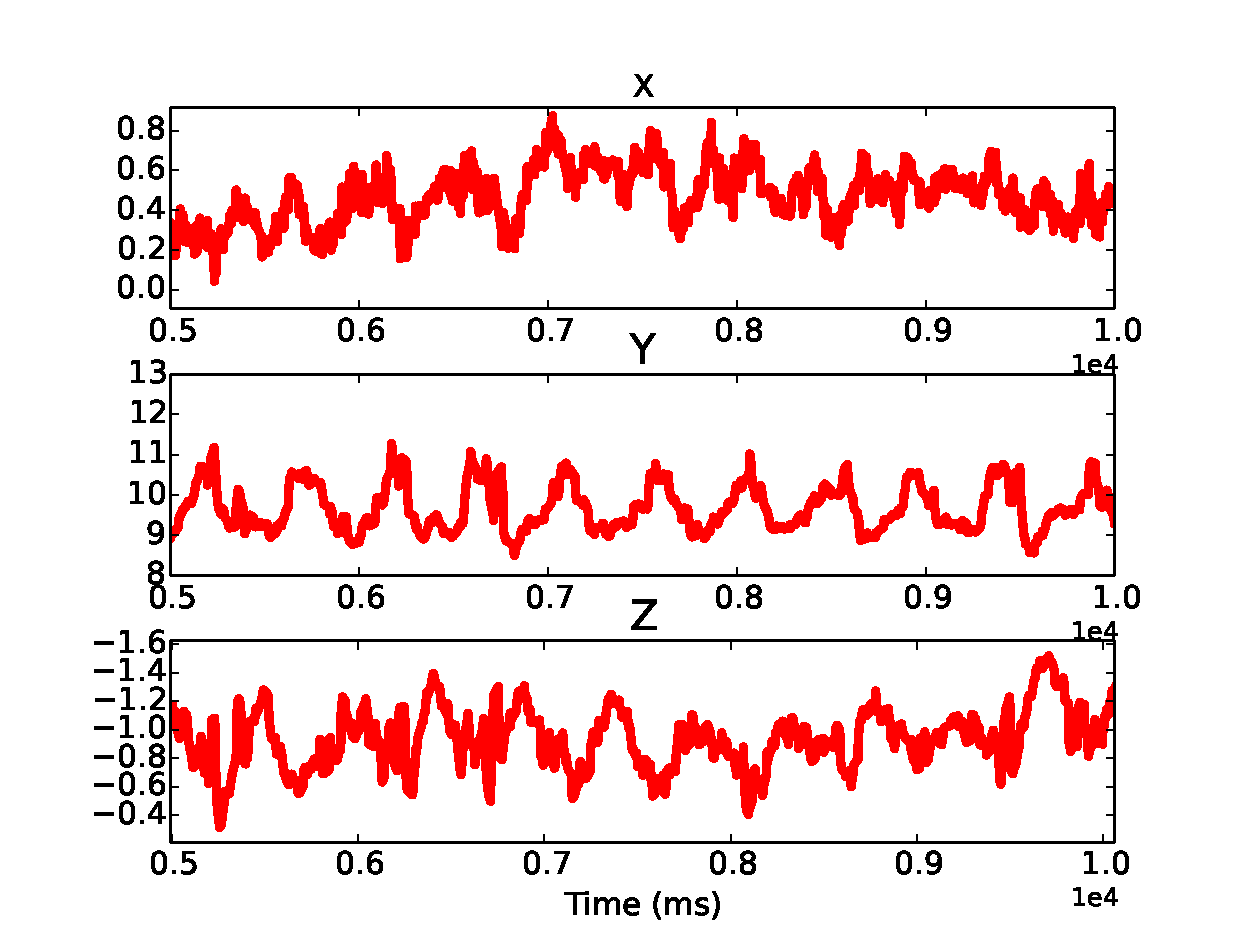
\includegraphics [width=.33\linewidth]{../mobisys_paper/fig/raw_sub4.eps}&
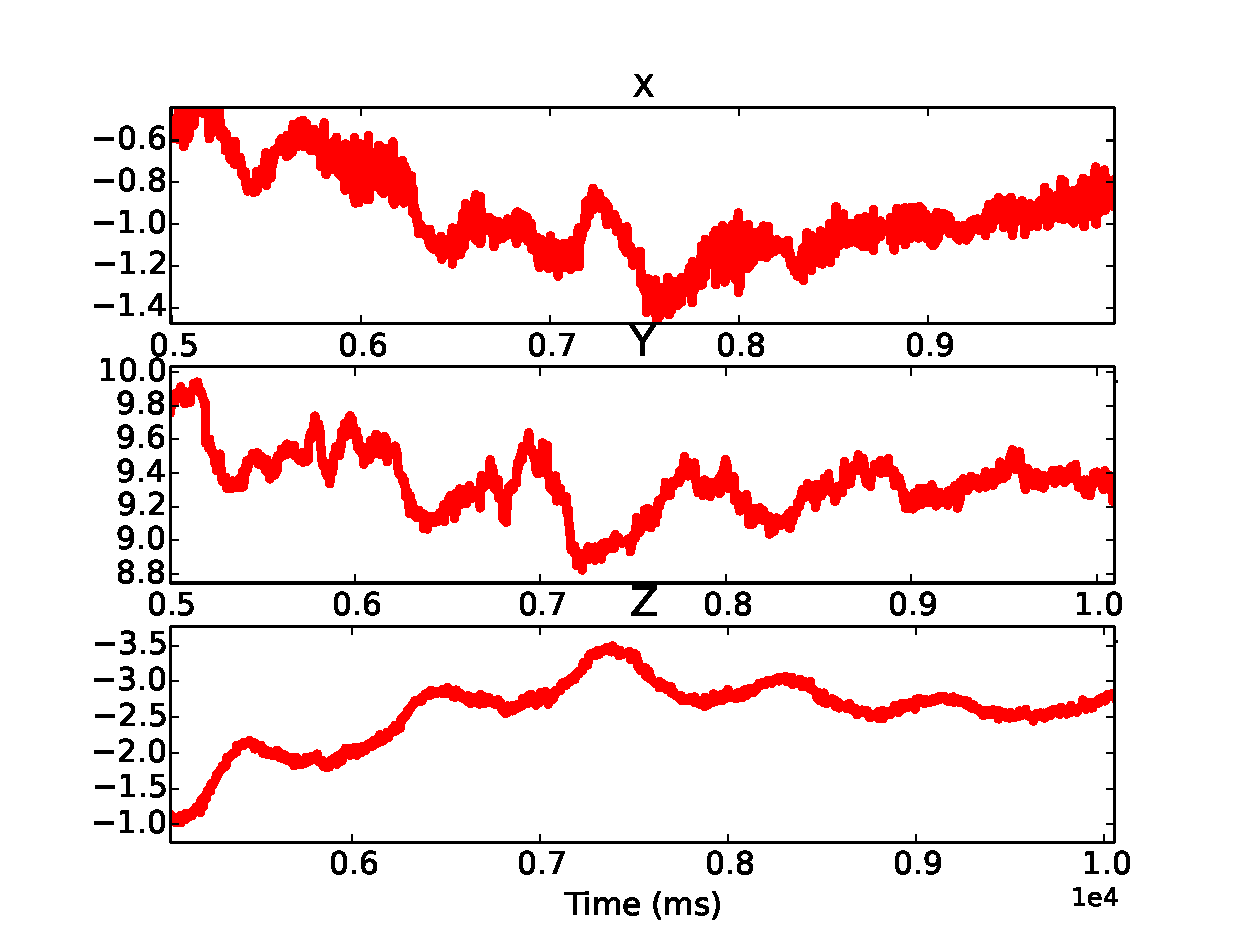
\includegraphics [width=.33\linewidth]{../mobisys_paper/fig/raw_sub5.eps}\\
(d) User 4& (e) User 5 \\
\end{tabular}
\end{center}
\caption{\label{fig:raw} These plots show the raw accelerometer data in the
time domain for five different users when they move their head in response to
a music track wearing the same Google glass. The plots
indicate that different users' head movement patterns appear distinctive from
each other. The five users wore a Google Glass (in turns) and listened to a
10 second audio snapshot of a pop song.}
\end{figure*}

\subsection{Background on Behavioral Biometrics}
%Authentication mechanisms for a wearable device can broadly be divided into two
%categories: (i) {\em Direct} authentication, where the users can directly
%authenticate themselves to their wearable device using the input/output
%interface and/or using signatures generated from the sensors available on the
%device, and (ii) {\em Indirect} authentication, where a secondary device --
%typically the user's smartphone -- is used as a medium for authentication.
%Today's commercially available wearable devices predominantly use the latter
%approach where users login to their wearable devices through their smartphone
%-- using a PIN or an email account.


%Unlike the indirect approaches, that require a wearable device is registered to
%and connected (wireless) to a smartphone, direct
%mechanisms can leverage the built-in interfaces and sensors on the
%wearable device.
Considering the fact that wearable devices relate significantly to ``what we wear" on the
human body, biometrics can play a key role for direct authentication to wearable
devices. Biometrics allow a system to identify a user based upon ``who you
are" (i.e., her physiology) instead of ``what you
have'' (i.e., ID cards) or `` what you remember'' (i.e.,
passwords)~\cite{jain2004introduction,o2003comparing,yampolskiy2007motor}.
Physiological biometrics such as DNA, ear shape, face, fingerprint,
hand/finger geometry,
iris, odor, palm-print, retinal scan, and voice, have been very effective and
widely used in many prototype and commercial authentication systems~\cite{wu1997measure,yan2007biometric,zhao1998discriminant,hong1998fingerprint,wildes1997iris,
yan2007biometric,baldisserra2005fake,hill2002retina,markowitz2000voice,reynolds2000speaker,bowyer2006survey,biddle2012graphical,sherman2014user,jain1997identity}.
In addition, body shape such as body height, width, and body-part proportions
can also be used as biometric cues to identify different
people~\cite{collins2002silhouette}. Even ``soft'' characteristics such as
body weight and fat percentage have been considered as secondary biometrics
for authentication purposes~\cite{ailisto2006soft}.

However, biometrics are
not prominently used in wearable devices commercially available today, though
there have been specific point commercial designs (e.g., Nymi~\cite{nymi}). This can be attributed to the
fact that biometrics would require the specific hardware/sensor available on
the wearable device. Also the overheads for physiological biometrics in
wearable devices can be high, in both, cost for hardware as well as
integration and computing.

Another approach to direct authentication is using behavioral biometrics
where unique signatures from human behavior (subconscious
or in response to external stimulus) provide cues for differentiating and
authenticating users. For example, it has been shown that gait (e.g.,
stride length, the
amount of arm swing) when the user is walking or
running is a reliable identification cue, and irrespective of the
environment~\cite{stevenage1999visual}. Okumura et.al.~\cite{okumura2006study}
have shown that the human arm swing patterns can be used to create signatures
to authenticate to their cell-phones. Monrose
et.al.~\cite{monrose2000keystroke} show that keystroke rhythms, when
users type on the keyboard, that include typing dynamics such as how
long is a keystroke, how far is between consecutive strokes, and how is the
pressure exerted on each key, can be used as a biometric to authenticate
users. Similarly, mouse usage dynamics~\cite{jorgensen2011mouse} and touchpad
touching dynamics~\cite{bo2013silentsense,de2012touch} have also been shown to
serve as potential biometrics.

In comparison to other means of authentication, behavioral biometric authentication can offer a more convenient (than physiological biometrics),
and more secure (than indirect authentication) solution for wearable device
authentication. With the increasing off-the-shelf availability and (almost) unlimited access to the motion sensors on the wearables, it
has become possible to generate and/or infer unique behavioral signatures
specific to users. We use these rationale as a motivation for our proposed
design of a behavioral biometric based authentication that generates unique
signatures from user's body movements. We design an authentication system, dubbed {\em Headbanger}, for wearable
devices by monitoring user's body-movement patterns (e.g., head movements, arm movements, and hand movements) in response to an
external music stimulus. Here, we do not limit body movements to pre-defined templates; rather, the user chooses \emph{free-style} movement she feels the most natural to do.
%\vspace{4pt}{\bf Head-movements as a behavioral biometric.}

\subsection{Body Movement as a Behavioral Biometric}
\label{subsec:headmovements}

%As such, authenticating a user involves comparing her sensor
%readings with the pre-recorded glass owner's sensor readings.
%Our design assumes that there is only one owner per glass, and we can easily
%extend our scheme to handle the cases with multiple owners.
%Figure~\ref{fig:sysarch} presents the system architecture of the \systemname,
%and in the following section, we will discuss each component of this design
%in more detail.

According to~\cite{jain2004introduction}, a human characteristic can be
considered as biometric as long as it is \emph{universal}, \emph{distinctive},
\emph{repeatable}, and \emph{collectible}. With the advancements in
wearable computer designs it is becoming easier for collecting body movement
patterns using the built-in sensors (e.g., accelerometer sensor, gyroscope sensor, motion sensor, etc). Such sensors are
available on most wearable devices available today, thus
making body movements that are both \emph{universal} and {\em collectible}.

In this proposal, we will show that free-style natural body movements are \emph{distinctive} and \emph{repeatable}, especially when combined with external stimuli such as music. In~\systemname, music plays a crucial role in stimulating body movements such that the resulting movement pattern is natural to the user (more distinctive) and easier to remember (more repeatable). It has been shown~\cite{zentner2010rhythmic} that most people move
their body as a natural response to external rhythmic stimuli such as music;
even at a very early age, infants respond to music and their movements speed
up with the increasing rhythm speed. Most adults naturally
perform head movements or hand movements when listening to a fast beat audio track.  When combined with external rhythmic stimuli, we believe body movements become more distinctive -- not only a person's movement pattern is unique, but her response to rhythmic stimuli is also unique. In this way, the resulting authentication system will be more dependable.

Before we go ahead and design our system, we first conducted a preliminary analysis of the accelerometer signals from five Google glass
users' head movements, and show the raw signals in Figure~\ref{fig:raw} (a)-(e). A quick glance at the raw signals reveals that these users
{\em repeatedly} showed unique and {\em distinctive} head-movement patterns, when listening to the same music beats on the head-worn device. Motivated by this observation we hypothesize that \emph{body movements can be a good behavioral biometric characteristic to authenticate
users to their smart wearable device}.
%We next formally present the design of our system that
%utilizes head-movement patterns as behavioral biometric signature

\vspace{4pt}\textbf{Example Body Movement Patterns:} Depending upon the wearable device to be authenticated, we can focus on the movements of different body positions. For example, head-mounted devices such as smart glasses can easily capture a user's head movement or eye lid movements; wrist-mounted devices such as smart watches can easily capture a user's arm/hand movements; shoe-based smart devices can easily capture a user's gait; smart rings can easily capture a user's finger/palm movements.

To facilitate natural and repeatable body movements, we can play short, fast-tempo music tracks on the wearable devices, and measure the resulting body movements using built-in sensors such as accelerometer sensor, gyroscope sensor, infrared sensor, etc.



\vspace{4pt}\textbf{Earlier Work on Body Movement Based Activity Detection and Authentication:} There have been a few point solutions that used body gesture/movements (captured by sensors such as accelerometers and gyroscope) for activity detection or authentication purposes. For example, Harwin et al.~\cite{harwin1990analysis} used head gestures (e.g., combining pointing and movements) for human computer interaction. Eye blinking pattern was looked at in~\cite{westeyn2004recognizing} as a unique feature for authentication. Ishimaru et al.~\cite{ishimaru2014blink} proposed to combine the eye blinking frequency from the infrared proximity sensor and head motions from accelerometer sensor on Google Glass to recognize activities (e.g., reading, talking, watching TV, math problem solving, etc).
Accelerometers have also been used for other parts of body movements for gait analysis, motion detection or user identification, such as waist~\cite{ailisto2005identifying}, pocket~\cite{gafurov2007gait}, arm~\cite{okumura2006study,gafurov2008arm}, leg~\cite{gafurov2006biometric,karantonis2006implementation,mantyjarvi2005identifying,derawi2010unobtrusive} and ankle~\cite{gafurov2011user}.
Hand gesture is often used to authenticate users on devices with touch screens.  A number of  features, including touch location, swipe/zoom length,
swipe/zoom curvature, time, and duration, have been exploited to authenticate smartphone or tablet users~\cite{sae2012biometric,frank2013touchalytics,cai2013mobile,feng2014tips,liu2009uwave,shahzad2013secure}.

\vspace{4pt}\textbf{How~\systemname~Is Different:} Compared to earlier point solutions that used simple/limited body movements or body gesture to authenticate users for smart phones or tablets, the unique constraints of wearable devices, combined with free-style natural body movements,  open up a completely new line of investigation in capturing body movement patterns, extracting unique user movement signature, and authenticating the user accordingly. Given the unique challenges of~\systemname, we will focus our investigation on the following two important questions: (1) Can we establish body movements as a biometric characteristic, and can sensors on wearable devices accurately capture the uniqueness of one's body movements? and (2) Can we run the body movement based classification algorithms on wearable devices without relying upon a second device?

\begin{figure}[t]
\centering
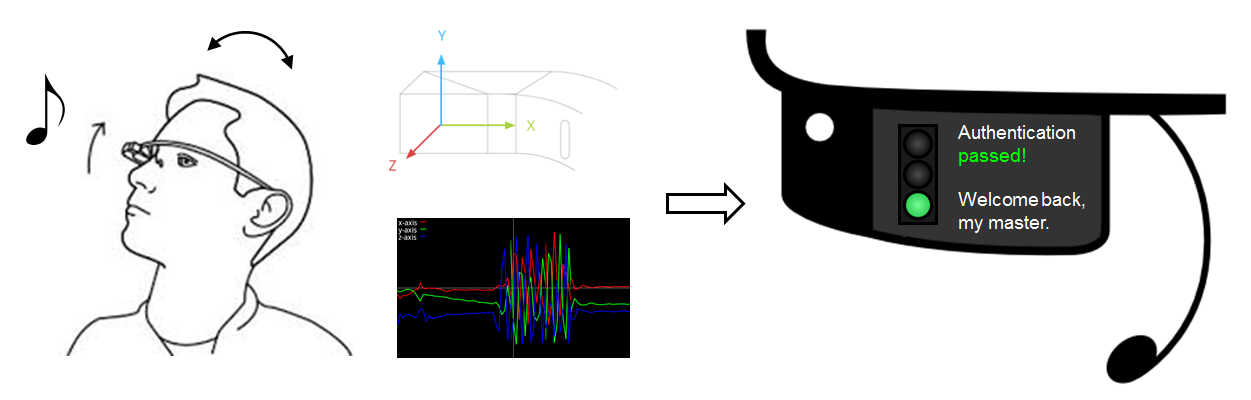
\includegraphics[width=.75\columnwidth]{../mobisys_paper/fig/headbanger-illustrate.png}
\caption{Illustration of Headbanger. The head-worn device authenticates the
right user based on signatures generated from head-movement patterns in
response to an audio snapshot played on the device.}
\label{fig:illustrate}
\end{figure}



\subsection{Overview of ~\systemname}

We refer to the proposed body-movement based authentication system tongue-in-cheek as~\systemname. We envision that~\systemname~will be used as an authentication interface on the wearable device, which will run upon device power-up, similar to the screen-lock in smartphones or the head-nod interface on Google Glass~\cite{googleglass}.  %~\systemname~keeps the real user's reference data and uses a classification approach to prove whether a user is the real user.

The authentication process has two parts: offline training and online authentication. In the offline training phase, the system collects the real user's body movement data and establish the features, which are referred to as \emph{reference} data. In the online authentication phase, we first ask the user to claim her ID from a list of user IDs (this can be done through simple gesture or voice). Next, we ask the user to pick a music track from a list of music tracks: if her pick does not match the claimed user's pick, then the authentication process exits immediately and returns FALSE. Otherwise,~\systemname~continues to go through the following steps:
\begin{itemize}
\vspace{-2pt}\item {\em Test sample collection}: In this step, we play the chosen music track for a few seconds (usually for up to 10 seconds), and ask the user to move along with the music. It is up to the user to decide which part of the body she will move(e.g., a combination of head, eye, arm, hand, leg, etc) and she will move. The advantages of using music as external stimuli are two-fold: (1) humans naturally respond to music beats by moving parts of their body, and (2) each person responds to music beats in different ways, and thus more user-specific information can be encoded in the movement pattern.

We record the raw sensor signals (e.g., from built-in accelerometer sensor or gyroscope sensor) during the music play period. We refer to the raw sensor data collected during a music track duration as a sample, e.g., an $ACC$ sample is the accelerometer data collected during the music period, and a $GYRO$ sample is the gyroscope data collected during the music period. After collecting the raw samples, we filter the samples to remove records of spurious motion so that the resulting sample will be much smoother and ready for subsequent processing.

\vspace{-2pt}\item {\em Classification}: In this step, we extract features from the filtered signal and run the classification algorithm against the reference data that was collected during the offline training phase. We will study a large set of features and classification algorithms and choose those that are suitable for wearable devices. If there is a plausible match, the user is accepted; otherwise, she is rejected.
\end{itemize}

Figure~\ref{fig:illustrate} illustrates the working of~\systemname. In this example, we try to authenticate Google glass users by monitoring their head movement patterns with music as external stimuli.


\subsection{Research Challenges}
Even though body movements have been used as biometric characteristics in other systems, it is completely unknown whether this method can be applied to wearable devices due to their unique constraints: (1) first, wearable devices are limited in battery/processing power and the types of sensors available to them, and (2) wearable devices should be able to deal with a much larger variety of body movements. Towards building a robust authentication system that solely runs on wearable devices, we strive to address two significant challenges in this project.

The first challenge is \emph{how we can establish body movement patterns as reliable biometric characteristics for authentication purposes.} In real life, it is common for us humans to recognize a person who is still far away by watching how she walks, i.e., her walking gait. To our brain, gait is unique, so are many other body movements. For example, by looking at how a person dances, we surely can recognize whether she is one of our friends.  However, 
whether the device we have, and/or the sensors available to the device, can capture, present, and quantify the uniqueness of these body movements, remains a challenge. The challenge is even more severe for seriously resource-constrained wearable devices and free-style natura movements. In this project, we will explore ways  to address this challenge. Towards this goal, we will find ways to pack as much as information in the sensor data, we will also try to authenticate users no matter they are stationary or walking, we will combine multiple movements that can be captured by a single wearable device, we will exploit multiple sensors to increase the authentication accuracy. For those users who desire a more secure authentication, we also exploit the fact that wearable devices can give out stimuli that only the wearer can feel to design body movement passwords which can greatly improve the authentication performance.

The second challenge is \emph{how we can minimize the resource consumption and processing delay of~\systemname~.} In order to achieve accurate classification results, it is often unavoidable to rely upon complex features and powerful classification algorithms, which will be very hard, if at all possible, to run on wearable devices. For this reason, wearable device authentication usually leverages a second device, which is much more powerful (e.g., smartphone). In this project, we take the viewpoint that authenticating users with two devices is inconvenient, and instead, we would like to implement the entire authentication process on the wearable device. To address this challenge, we propose to carefully choose the features and classifiers, and more importantly, we propose to pipeline the online authentication operations to significantly reduce the latency and power consumption. Finally, we also propose to dynamically adjust the sampling rate based upon the physical context information about the device.

\section{Challenge I: Establishing Body Movement Patterns as Reliable Features for Authentication}\label{sec:learning}

Even though body movements have been deemed unique by human brains for a long time, the need to capture the signal and quantify its uniqueness using wearable device is highly challenging. In this section, we present our proposed techniques to address this challenge.

\subsection{Preliminary Results}
We have conducted a preliminary study to find out whether body movements measured by wearable devices can potentially be used for robust authentication.
In our preliminary study, we used Google glass to collect accelerometer data ($ACC$ in short) when a user moves her head following music beats, and studied whether the measured head movement patterns are distinctive and repeatable. Our preliminary study involves the following data processing aspects:

\begin{enumerate}
\vspace{-2pt}\item \emph{Filtering}: Since the frequency spectrum of the $ACC$ samples is significantly concentrated within 5Hz, we filtered the raw samples using a low-pass digital Butterworth filter~\cite{challis1983design} by adopting a relaxed cut-off frequency of 10Hz. In this way, we removed spurious head movements and obtained smooth $ACC$ data.

\vspace{-2pt}\item \emph{Reference Data Construction:} We constructed the reference data set to include $m$ $ACC$ samples from the legitimate user (which we refer to as \emph{true} $ACC$ samples), as well as $m$ $ACC$ samples each from $N$ random users (referred to as \emph{false} samples). Then we calculated the distances between these samples using the dynamic-time warping (DTW) tool~\cite{dtw}\footnote{DTW is generally used to measure similarity between temporally varying signals. DTW compares a temporal signal with a reference signal over a certain time-window and calculates the distance between these two signals.}. Using DTW, we calculated the distances between true $ACC$ samples and the distances between true samples and false samples, and refer to these two types of signatures as same-user distance signatures as well as across-user distance signatures. In general, we find that same-user distances are much smaller than cross-user distances. 

\vspace{-2pt}\item \emph{SVM Classification:} In the online authentication phase, after filtering the raw $ACC$ signal, we calculated the DTW distances between the test sample and the true samples, and then feed these distance values and the reference data to the Support Vector Machine (SVM) to obtain classification results. %SVM returns '1' to denote that the test user is accepted and '0' to denote the user is rejected.

\end{enumerate}


\begin{table}[b]
\centering\small
\begin{tabular}{|l||l|l|l||l|l|l||l|l|l||l|l|l|}\hline
& \multicolumn{3}{|c||}{2}& \multicolumn{3}{|c||}{3}& \multicolumn{3}{|c||}{6}& \multicolumn{3}{|c|}{10}\\\cline{2-13}
Sample duration (s)& FRR & FAR & BAC & FRR & FAR & BAC & FRR & FAR & BAC & FRR & FAR & BAC\\
&(\%) &(\%) &(\%) &(\%) &(\%) &(\%) &(\%) &(\%) &(\%) &(\%) &(\%) &(\%)\\\hline

SVM          & 25.0 & 16.74 &79.12 & 15.0 & 14.05 & 85.47 & 3.33& 6.66& 95.0  & 0.0& 9.62& 95.18\\\hline

\end{tabular}
\caption{Average FAR, FRR, and BAC for SVM-based classification in our preliminary study. The results show that even for the simplest nodding, we can correctly authenticate 95\% of the users when the samples are longer than 6 seconds. \label{tab:kfoldfalse-svm}}
\end{table}


\vspace{4pt}\textbf{Distinctiveness:} We designed the first set of experiments to show that even the simplest head movements are distinctive -- i.e., it is hard to imitate other's movement patterns. In this set of experiments, we employed the simplest head movement pattern: nodding. In total, we had one glass owner, who designed the nodding pattern, and 15 imitators who imitated the pattern. We collected 100 10-second $ACC$ samples from the owner, during the course of 60 days (from 10/1/2014 to 11/30/2014), ensuring the owner's sensor data includes sufficient variation that naturally arises with time. We also made a great deal of effort to make sure the imitators accurately copy the owner's movement -- the owner carefully explained how he nodded his head to each imitator, and sat through each data collection session for all the 15 imitators to make sure their nodding patterns look the same to the owner's eye. For each imitator, we collected 40 10-second $ACC$ samples. By averaging over many different combinations of reference data and test data, we generated the average classification results and summarized the mean FAR (false acceptance rate), FRR (false rejection rate), and BAC (balanced accuracy) in Table~\ref{tab:kfoldfalse-svm}. The results show that \emph{even simple nodding is not easy to imitate: nodding for 6 seconds can help classify 95\% of the users.} %As the sample duration increases from 2 seconds to 6 seconds, the classification accuracy improves significantly -- the BAC value changes from 79.12\% to 95\% for top 1 testing, and from 87.95\% to 93.27\% for top 3 voting. After the sample duration reaches 6 seconds, the improvement becomes less pronounced. This suggests that a sample duration of 6 seconds is sufficient to successfully classify 95\% of the users. We feel that moving our head gently along with music for 6 seconds is in general not a cumbersome process for most users. It further suggests that even simple nodding is hard to imitate by others, and thus head-movement has the potential to %serve as a reliable biometric characteristic for smart wearable authentication.

\begin{figure*}[t]
\centering
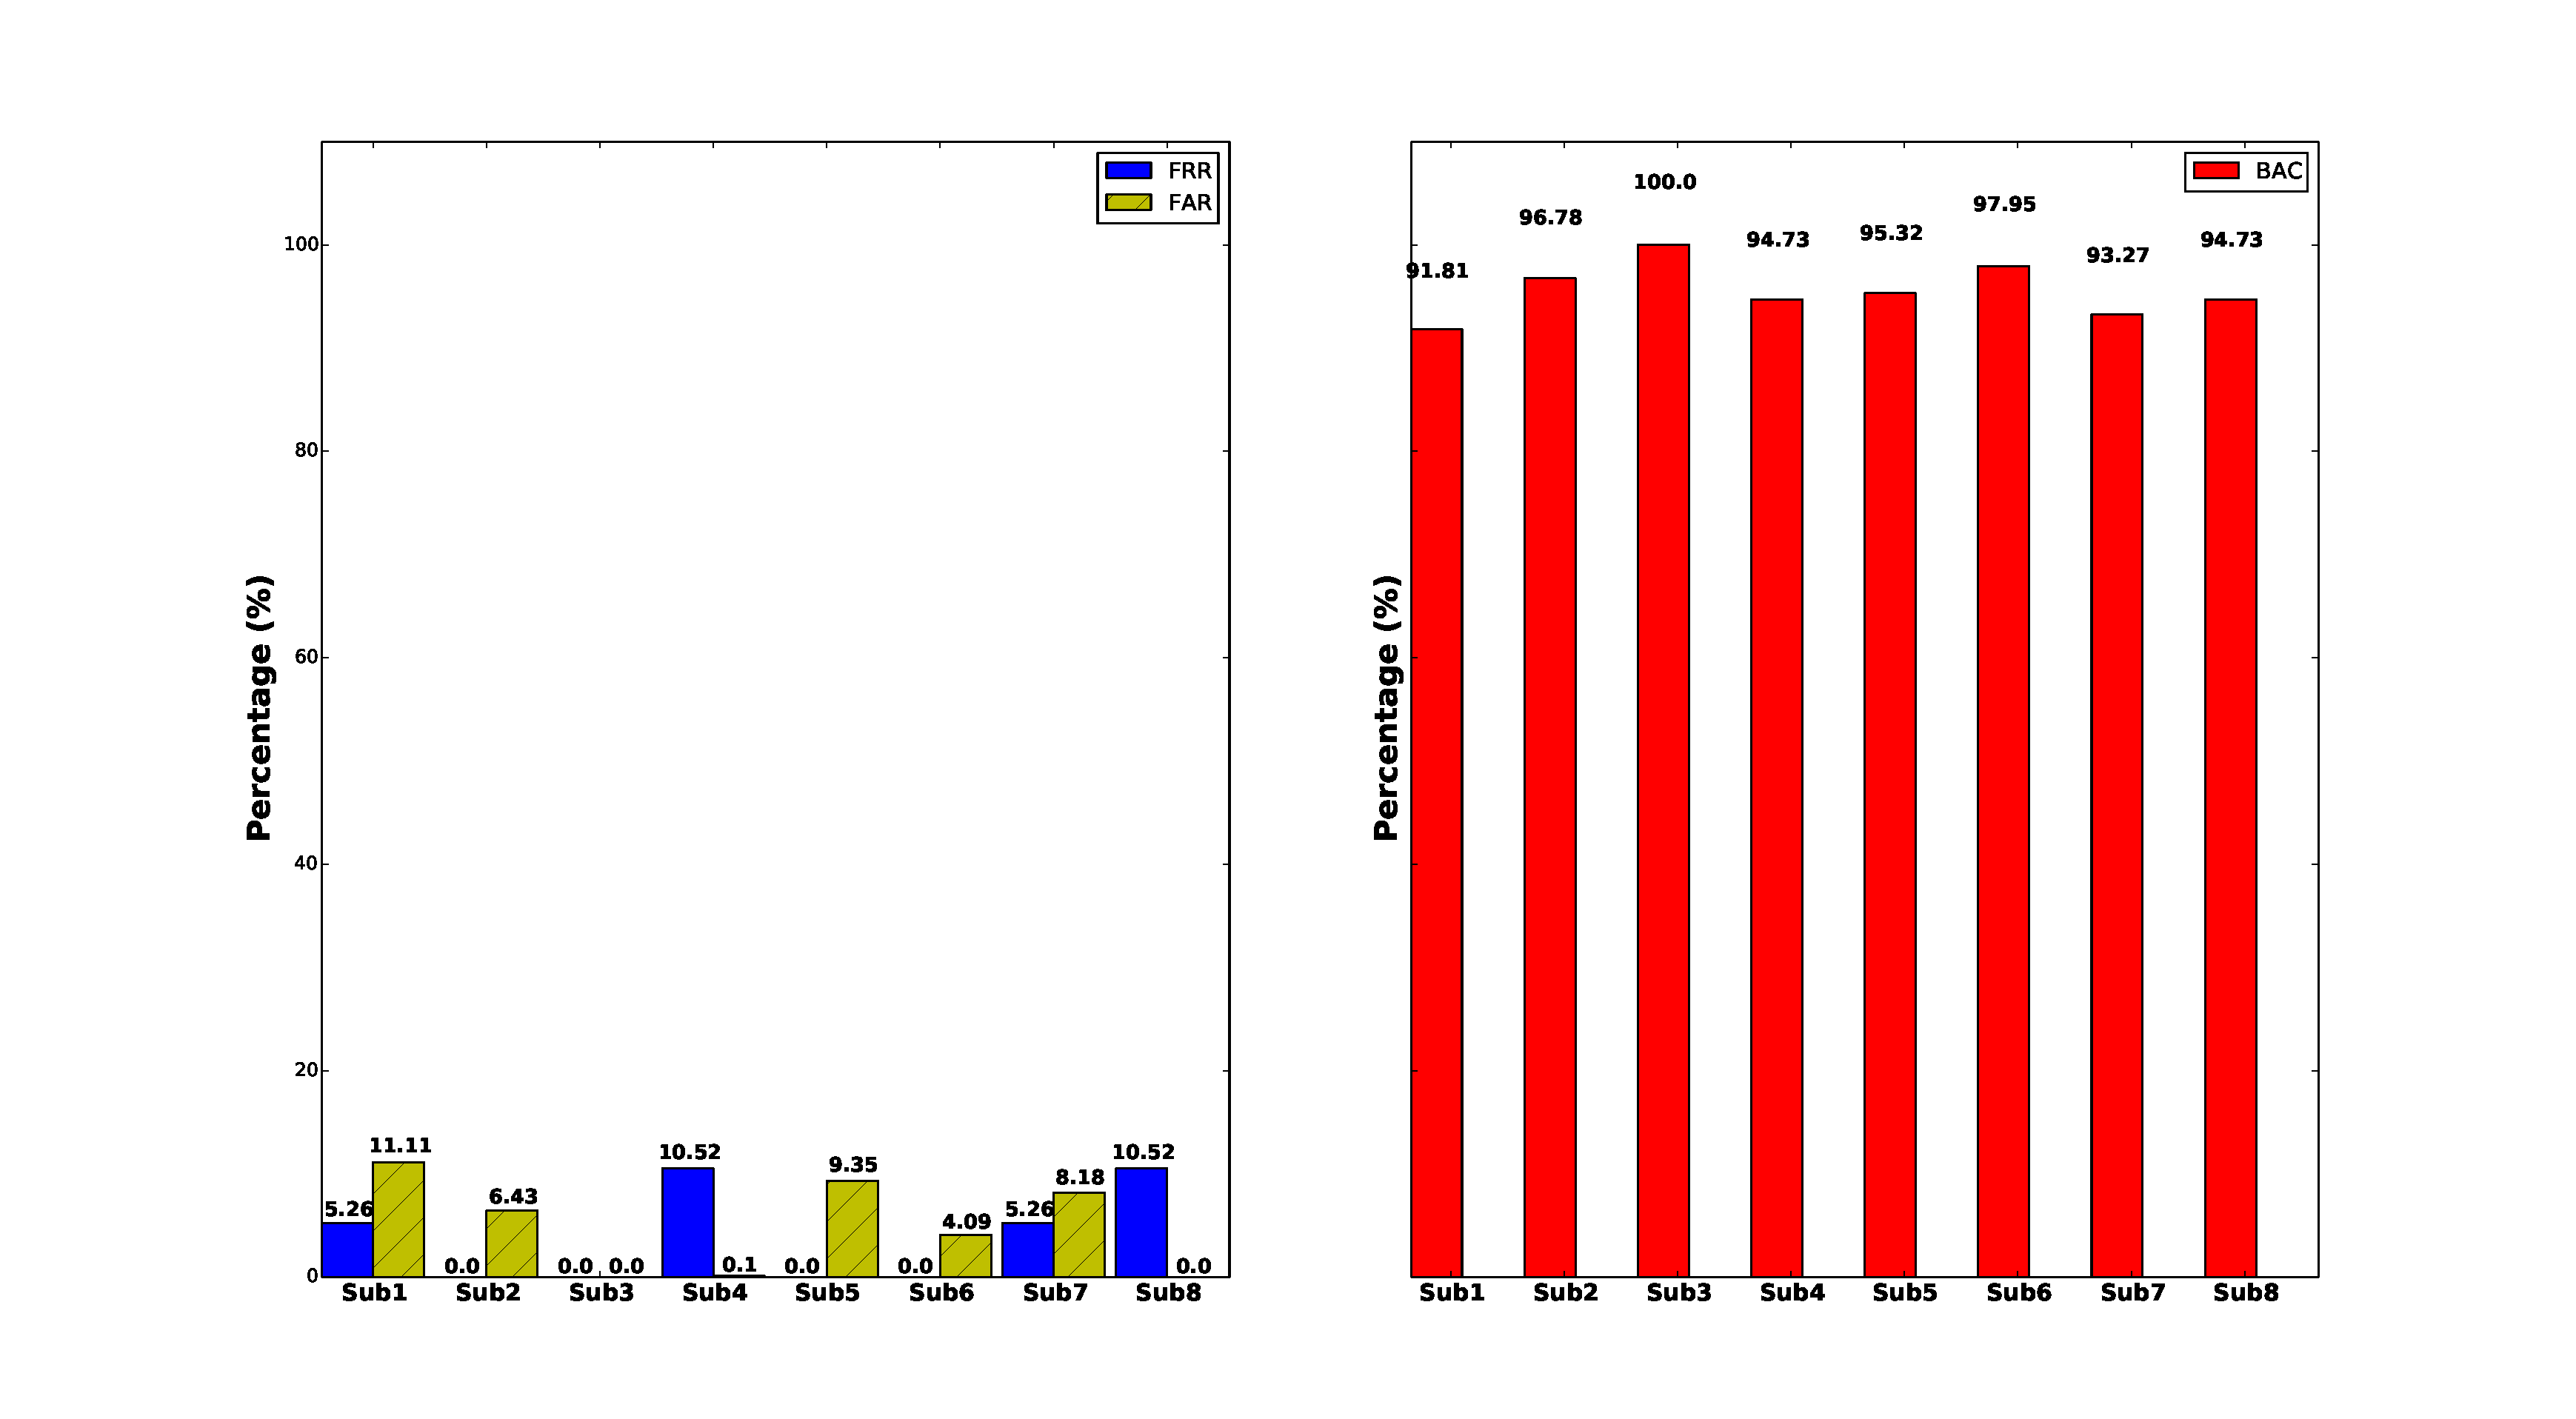
\includegraphics [width=.75\linewidth]{../mobisys_paper/fig/exp2_frr_far_bac.pdf}
\caption{In this set of experiments, we studied whether a user can successfully repeat her own head-movement pattern. We had 8 subjects, each performing her own choice of head-movement patterns. We collected 38 samples for each subject. (a) shows the FRR and FAR results for each subject, and (b) shows the BAC results.\label{fig:exp2_frr_far_bac}}
\end{figure*}

\vspace{4pt}\textbf{Repeatability:} We designed the second set of experiments to show that a user can successfully repeat her own head movement pattern if each user is asked to come up with their own movement pattern. In this set of experiments, we had 8 subjects, and for each subject, we collected 38 $ACC$ samples with sample duration of 10 seconds. Each subject performed different head-movement patterns of their choice. We report the average FAR, FRR, and BAC values in Figure~\ref{fig:exp2_frr_far_bac}, where Figure~\ref{fig:exp2_frr_far_bac}(a) shows the FRR and FAR values, while Figure~\ref{fig:exp2_frr_far_bac}(b) shows the BAC values. The results show that \emph{head-movements are highly repeatable.} Among the 8 subjects that we studied, the highest BAC value is 100\%, and the lowest is 91.81\%, with the average BAC value of 95.57\%.

%Overall, our preliminary results suggest that the head movement pattern is a very promising biometric candidate for wearable user authentication.

\subsection{Proposed Research}
Our preliminary results show that simple movement patterns have the potential to be used as a reliable biometric characteristic for wearable user authentication. However, in order to develop a full-fledged authentication system using free-style body movements, we need to eliminate several important roadblocks.

\subsubsection{Feature Selection and Information Entropy}\label{sec:feature}
Feature selection plays the most important role in determining the accuracy of an authentication system, and we will thus start our discussion from this topic.  Most wearable devices have accelerometer ($ACC$) and gyroscope ($GYRO$) sensors, whose readings can be used to characterize a person's body movements. There has been a long history of studying these two types of sensor data to detect/analyze motion, and a large number of features have been discussed~\cite{palmerini2011feature,Pirttikangas2006feature,preece2009comparison,bao2004activity,zhang2011feature}. In this project, we will start our investigation by evaluating these features, and propose to look at the following features in depth: (1) mean, standard deviation, median, 25\%, and 75\% of frequency (in the frequency domain), (2) mean low and mean rectified high pass filtered signals (in the frequency space), (3) centroid frequency (in the frequency domain), (4) frequency dispersion (in the frequency domain), (5) power spectrum of entropy in acceleration/rotation and average energy in acceleration/rotation (in the frequency domain), (6) magnitude of first five components of FFT analysis (in the frequency domain), (6) jerk index that indicates the smoothness of the signal (in the time domain), (7) mean crossing (in the time domain), (8) maximum difference acceleration (in the time domain), (9) correlations between axes (in the time domain). We will conduct an in-depth comparison of these features, and select those that deliver the best performance; meanwhile, we will also design new features that are suitable for our study.

\vspace{4pt}\textbf{Boosting Information Entropy:} It is important to encode as much information as possible into the observed sensor signals to achieve higher information entropy. One way of achieving this goal is to have the user move her body naturally following an external music stimulus -- we hypothesize that different people translate music stimuli to motor movements in different ways~\cite{bartenieff1980body,brass2001movement,dassonville2001effect}. For example, some people are able to follow beats much closer than others, some can follow beats more regularly than others, etc. By using the music stimuli, in addition to the afore-mentioned baseline $ACC$/$GYRO$ features, we can also consider a group of new features concerned with the temporal relationship between music beats and subsequent body movements --  such as mean and standard deviation of the intervals between a music beat and the subsequent body movement, the top interval values, etc. In this way, the sensor data contains more information than just the movement pattern.

In order to further boost the information entropy, we can also switch the music track during a data collection session. In this way, the sensor data does not only contain the user's motor response to the music beats in a steady state, but it also encodes information about how fast the user adapts to the change of music rhythm, which provides more discrimination power.

\subsubsection{User Authentication Through Combined Movements and Sensors}

Smart wearable devices typically contain an array of motion sensors such as accelerometer, gyroscope, and inertial measurement unit (IMU). It is only a matter of time that motion sensor chips will be integrated into wearable devices.
This opens up opportunities for multi-modal motion sensing. For example,
accelerometer data can be combined with gyroscope measurements to provide
multi-dimensional movement features that can improve the quality of the
inferred signatures. Head movements can also be combined with other body movements to generate
valuable, reliable signatures for authentication. In this project, we plan to explore these opportunities.
%Additionally, head-movement is just one type of body movements, and we can
%investigate other types of body movements as well.


\begin{wrapfigure}{r}{3.0in}\centering
\vspace{-12pt}
\begin{tabular}{cc}
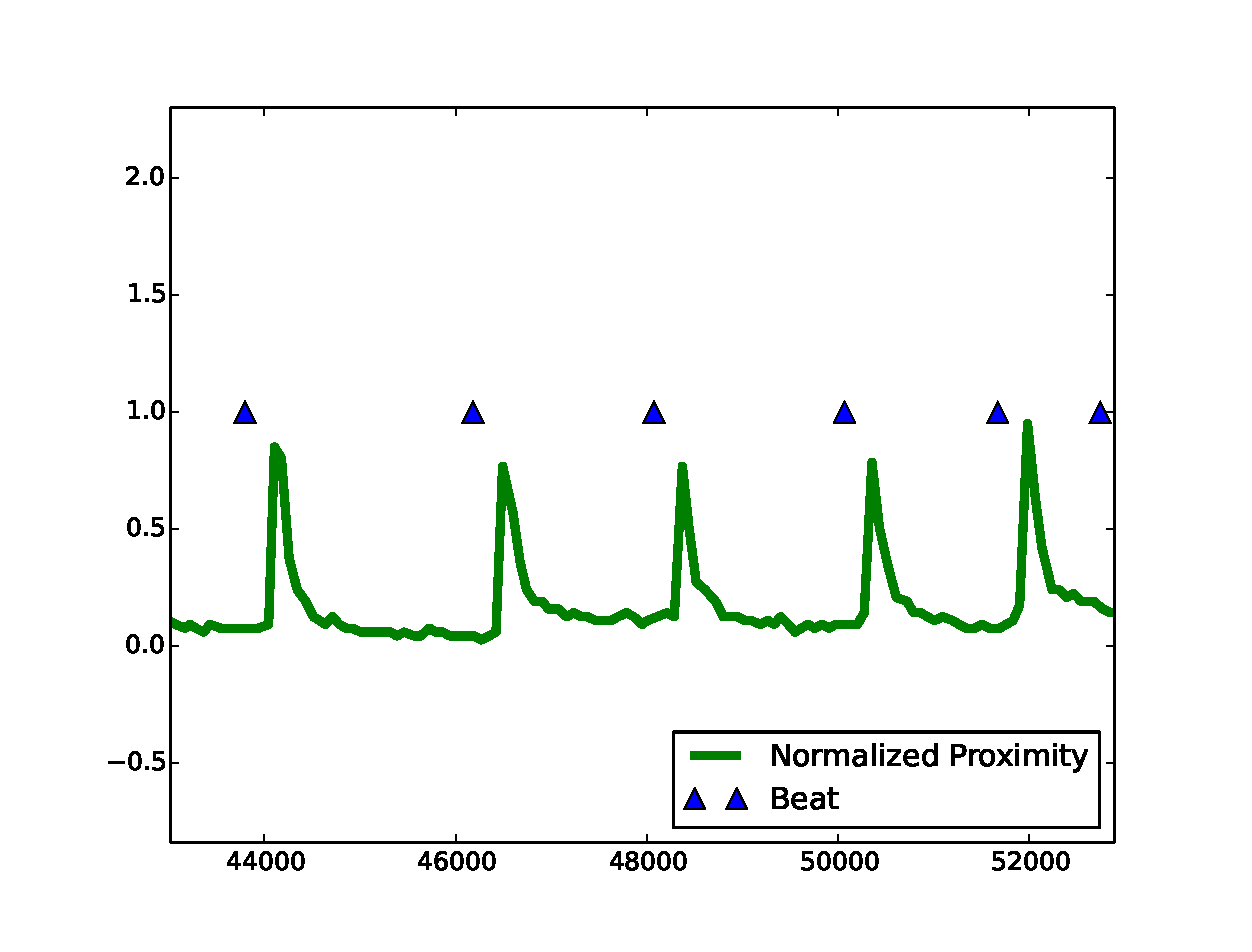
\includegraphics[width=0.50\linewidth]{../figure/sub1_blink_beat} &
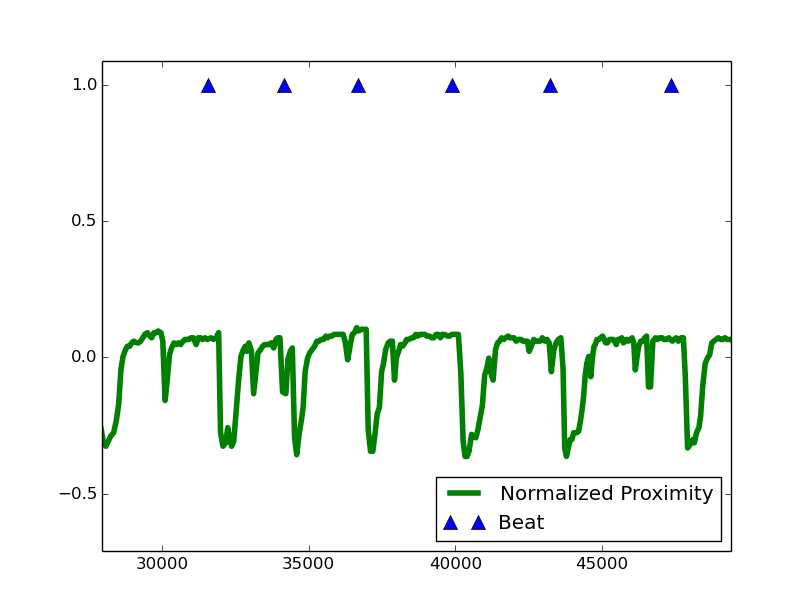
\includegraphics[width=0.50\linewidth]{../figure/sub2_blink_beat} \\
(a) & (b)\\
\end{tabular}
    \caption{\label{fig:blink} A person's blinking patterns (measured by the infrared proximity sensor on the Google Glass) with respect to music beats are also differentiable.}
\vspace{-12pt}
\end{wrapfigure}
\vspace{4pt}\textbf{Combining Multiple Movement Signatures:} In our preliminary study, we only looked at monitoring head movements for authenticating Google Glass. In reality, there are other types of movements that can be captured by Google Glass for authentication purposes. For example, through a simple test experiment using the Google Glass
infra-red light sensor we observed that the blinking and winking patterns of users in
response to the music can be combined with head-movements for better results. For example, Figure~\ref{fig:blink} shows two users' blinking pattern (captured by the infra-red light sensor, or the proximity sensor) with respect the music tones are vastly different. Recent studies have also shown that heart beat or pulse can be read by Google Glass~\cite{hernandezbioglass}. In this project, we will look at whether these signals can be combined to obtain better classification results.

The main challenge in combining multiple movements stems from the fact that it is hard to separate their impacts on motion sensor readings (e.g, the fact that a user winks may change the way she moves her head). As a result, if not properly handled, combining movements may actually worsen the authentication results. In this project, we will carefully investigate what new features we will exploit if multiple movement patterns are combined.

\vspace{4pt}\textbf{Combining Accelerometer and Gyroscope:} Quite a few previous studies have looked at combining accelerometer and gyroscope readings to detect motion contexts such as walking, standing or fall~\cite{mayagoitia2002accelerometer,jovanov2005wireless,li2009accurate,zhu2004real,williamson2001detecting,sabatini2005assessment}. In our preliminary study, however, we find that gyroscope data from Goolge Glass fared very poorly in discriminating users' head movements. The reason is that gyroscope often drifts over time. Low pass filtering can help cancel such drifts, but it also erases much useful information in the low frequency range, thus rendering it less useful. On the other hand,  complimentary filters (discuss in~\cite{euston2008complementary}) that combine accelerometer and gyroscope readings could provide attitude estimation. It performs low-pass filtering on a low-frequency attitude estimation that is obtained from accelerometer, and high-pass filtering on a high-frequency attitude estimation that is obtained by the integration of  gyroscope data. Though better than low-pass filtering alone, this may also lead to information loss in the low frequency range, hence poorer classification results. In this project, we will try to develop a signal processing method that can better preserve information in the low-frequency range.

\vspace{4pt}\textbf{Authenticating Multiple Devices:} When a person has multiple wearable devices, we don't need to authenticate the same user to different devices one by one (assuming these devices are not put on at the exactly the same time). Instead, after the user is authenticated on the first device, the first can help the user authenticate on the second device by having the user make simple and short body movements that can be measured by both devices (e.g., shaking two devices using one hand each)~\cite{mayrhofer2007shake,patel2004gesture}.


\subsubsection{Robust Authentication in Mobile Settings}
Our preliminary results show that head movements are rather distinctive and repeatable in very controlled settings -- all the data were collected when the participant was in a stationary setting, i.e., sitting on a chair. However, in reality, the behavior of body movement signatures over chaotic settings will be a key factor to decide on the effectiveness of this approach. In this project, we strive to solve the challenge for the most common mobile setting: when the user is walking.
%Our work only evaluates the case when a
%user is in a stationary setting when attempting to login, such as when sitting
%on the chair or standing still. The performance of this approach in realistic


\begin{wrapfigure}{r}{4.0in}\centering
\begin{tabular}{cc}
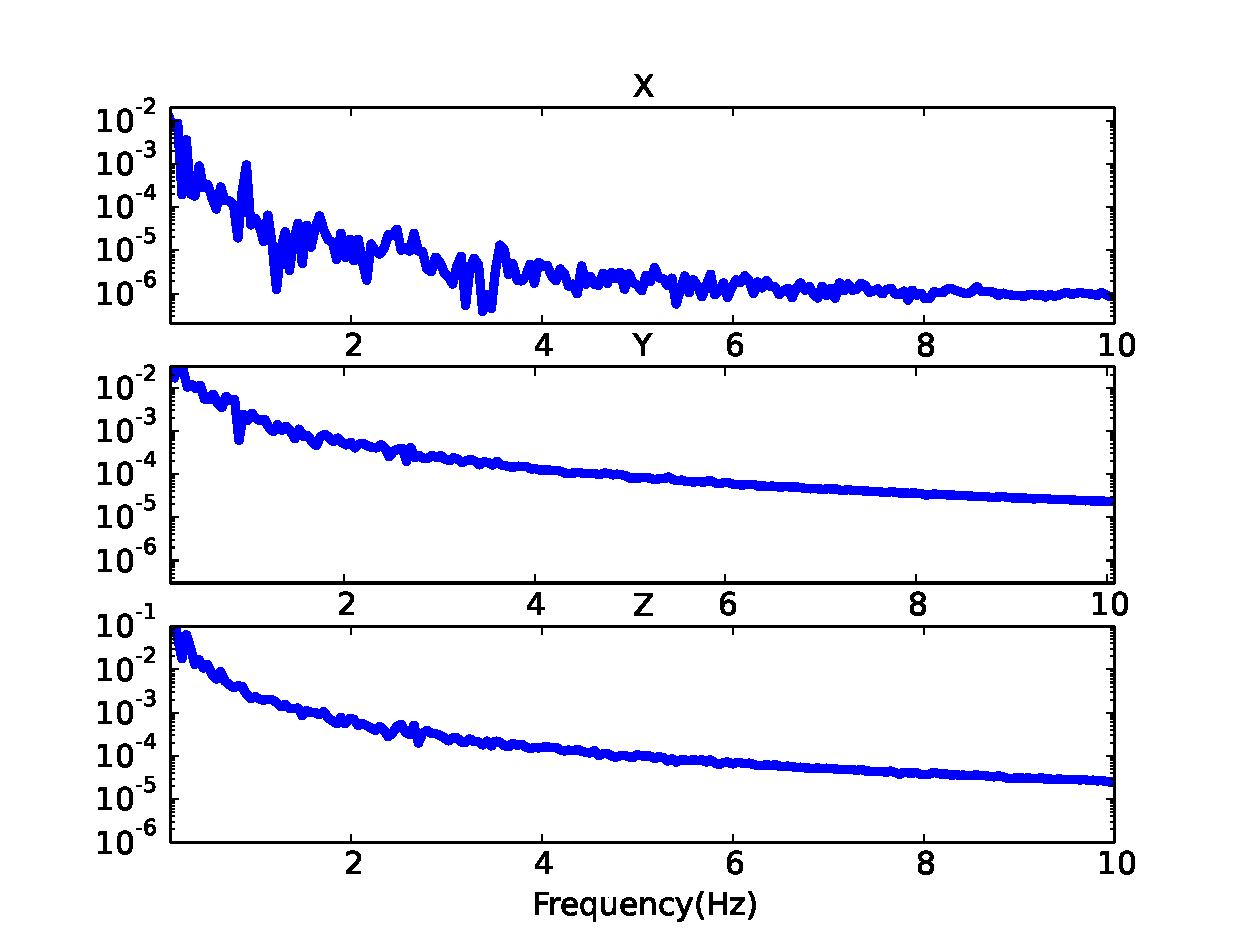
\includegraphics[width=0.50\linewidth]{../figure/sub1_walking_freq} &
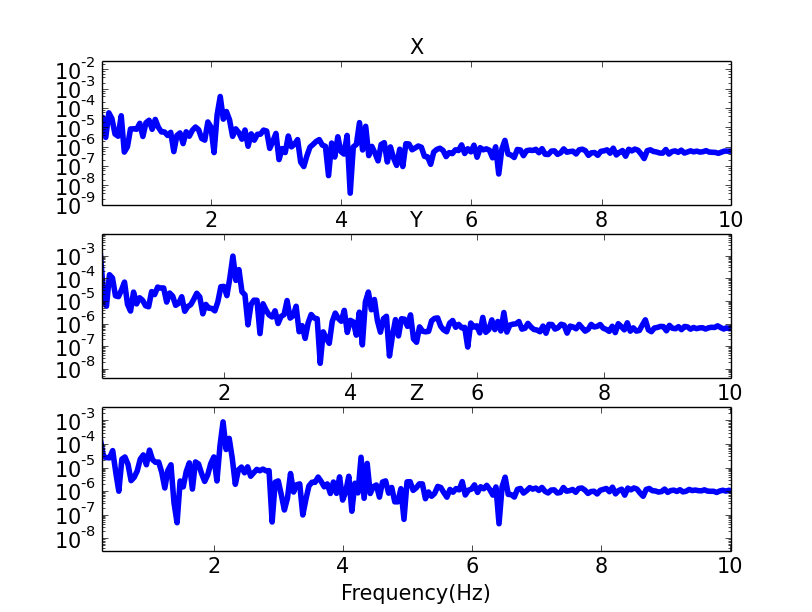
\includegraphics[width=0.50\linewidth]{../figure/sub1_nodding_freq} \\
(a) & (b) \\
\vspace{-4pt}
\end{tabular}
    \caption{\label{fig:walk} Walking (a) usually has more energy than music-stimulated partial body movement such as nodding (b).}
\vspace{-6pt}
\end{wrapfigure}
\vspace{4pt}\textbf{Authenticating Walking Users:}  For a walking user, we can't rely on the original training data that is collected when the user was sitting or standing still any more; performing body movements while walking will definitely lead to different movement signatures.

When considering walking, we can collect sensor readings in three different scenarios (we only focus on $ACC$ data in this part for the sake of simplicity): ${ACC_{M+W}}$, denoting the sensor readings when the user is performing body movements while walking; ${ACC_{M}}$, denoting the sensor readings when the user is performing body movements while sitting or standing still; and ${ACC_{W}}$, denoting the sensor readings when the user is walking, without any special body movements. To address the challenge of authenticating walking users (whose test data is $ACC_{M+W}^{tst}$), a naive
method is to use an external accelerometer (such as the one on the smartphone) to record the motion caused by walking ($ACC_{W}^{tst}$). We can then extract the motion caused by special music-stimulated body movements as $$ ACC_{M}^{tst} = ACC_{M+W}^{tst} - ACC_{W}^{tst}.$$ Finally we can compare $ACC_{W}^{tst}$ with the reference data $ACC_{W}^{ref}$ to classify the user. Though simple and effective, this method does require another device, which is less convenient, as we have argued before. As a result, we will \emph{not} adopt this method in the project.


If we only use the accelerometer on the device, authenticating a walking user becomes much harder, mainly because a person's walking pattern is much less repeatable -- factors such as trajectory, speed, terrain will have a bearing on the walking pattern -- and the interaction between walking and music-stimulated body movements are very complex and hard to predict. Due to the complexity of this problem, we will explore a learning-based authentication approach. In the learning phase, the system will ask the user to perform the designed body movements while she is in different walking contexts (walking in office, walking at home, walking on the parking lot, etc.). The system will then run clustering algorithms on the collected accelerometer data, and cluster them into a small number of groups, representing the data within her typical walking contexts. For each such group, we maintain a certain number of reference data.

In the classification phase, we adopt a two-level classifier. At the top level, we determine whether the user is stationary or mobile. This is rather straightforward because walking in general has much more energy than music-stimulated body movements as shown in Figure~\ref{fig:walk}. At the bottom level, if the user is walking, we classify the test data against the user's walking reference data group by group. If none of the groups return TRUE, we reject the user.


\subsubsection{Stronger Authentication Through Body Movement Based Passwords}\label{subsec:password}
Like any behavioral biometric characteristic, the body movement pattern may fail to differentiate users in some cases. For those users who desire a more secure authentication method, we propose to use movement-based passwords, which offers more security, reduces the processing demands on the device, but requires the user to remember their passwords.

Like traditional text passwords, body movement passwords also contain a list of elements -- how many elements are in the password and what they are determine the password. However, unlike tradition passwords in which each element is a character, each element of the body movement passwords is a type of body movement. For example, a password for a smart glass user can have the following four movements: a head nod, an eye blink, a head nod, and a head shake; a password for a smart watch user can have the following four movements: upward movement, right-award movement, left-award movement, and downward movement. For each element, the system also designs a unique prompt tone that the user needs to remember. 

The proposed password-based authentication system works as follows. First, we ask the users how many elements are contained in her password. Then for each element, the system will play a tone to mark the beginning of the element. We make sure two consecutive tones will be reasonably apart so that the user has sufficient time to finish each movement. In this case, the system doesn't need to differentiate users solely based upon their movement signatures, but the system only needs to recognize the movement. We will also provide a list of supported movements such as a head nod, a head shake, or an eye blink. Finally, for each authentication session, the system plays the prompt tones in a \emph{random} order to avoid shoulder surfing. Compared to using body movements as biometrics, this method is simpler, more secure, and easier to reconfigure than purely movement pattern based authentication. 



\section{Challenge II: Building an Efficient Body Movement Based Authentication System}\label{sec:system}


The second challenge we will deal with in this project is to ensure the proposed authentication system can run on seriously resource-constrained wearable devices. Our preliminary results show that even a highly simplified classifier will incur high processing latencies, sometimes leading to the catastrophic device overheat exception. To tackle this challenge, we propose to carefully select efficient features and classifiers, pipeline the authentication operations, and dynamically adapt the sampling rate.

\subsection{Preliminary Work}
\begin{wrapfigure}{r}{3.0in}\vspace{-12pt}
\centering
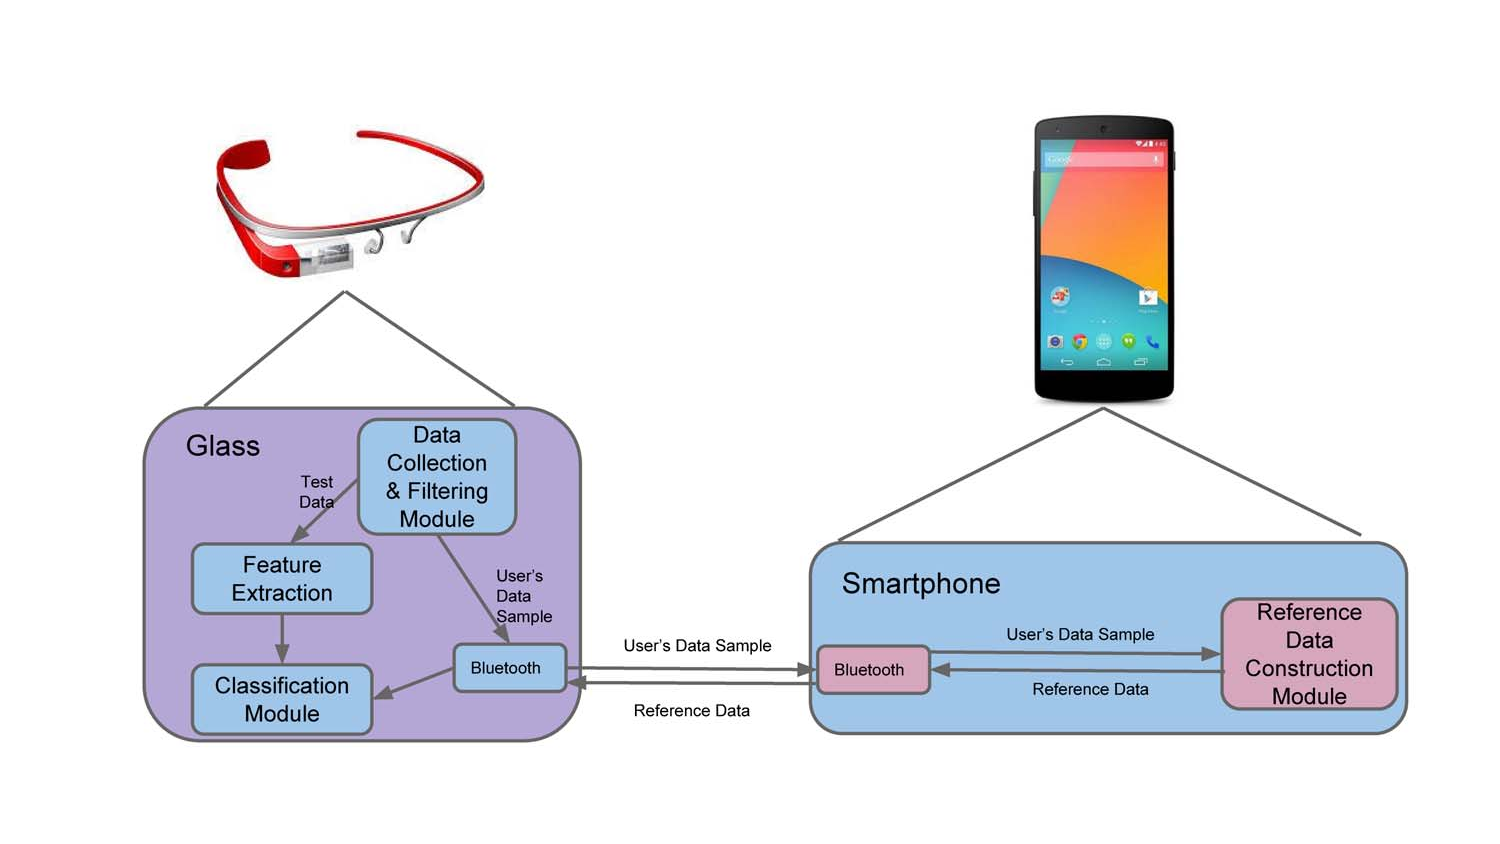
\includegraphics [width=.9\linewidth]{../figure/sofware_architecture}
\caption{The software modules for the Headbanger authentication app we implemented in the preliminary study. \label{fig:software_arch}}\vspace{-12pt}
\end{wrapfigure}
Wearable devices have severe resource limitations in many aspects; to name a few, energy, computing, networking and storage. Building an efficient authentication system that can smoothly run on such devices, therefore, becomes a significant challenge. In order to investigate whether such a goal is attainable, we have implemented a ~\systemname~app on the Google Glass. Figure~\ref{fig:software_arch} shows the software modules the app consists of. In the implementation, we established the reference data on the smartphone since this step is offline, consumes the most resources, and doesn't need to run on the device. The online
authentication process is implemented on the device. In the implementation, we adopted a much simplified classification method. First, instead of having multiple reference samples, we only use one reference sample for each user. After computing the DTW distance between the test sample and the reference sample, we simply compare the distance to a pre-set threshold value to determine the classification result. In this implementation, we kept the algorithm to the bare minimum to test the processing capability of the Google Glass and did not worry about the classification accuracy.

\begin{wrapfigure}{r}{3.0in}\centering
\small\centering
\begin{tabular}{|l|l|}\hline
sample  & processing \\
duration (s) & delay (s) \\\hline
2 & 1.29 \\\hline
3 & 2.74 \\\hline
6 & 9.04 \\\hline
10 & 20.48 \\\hline
\end{tabular}
\caption{\label{tab:glass}Measured processing latencies on Google Glass with different sample durations. In this set of experiments, we tried to understand the processing capability constraints and didn't optimize the code. }
\end{wrapfigure}
Figure~\ref{tab:glass} shows the measured processing latency (the time that elapsed between when we finish collecting the test sample and when the authentication result is generated). The results show that even with a significantly reduced implementation, the processing delays are still rather substantial. For example, if the sample duration is 10 seconds, the processing delay is a little more than 20 seconds! More importantly, if there were other processes such as camera running at the same time, or if we continuously ran the~\systemname~app for multiple times, then the processing became very slow, and the glass became overheated and displayed the following message ``It is too hot. Glass needs to cool down.'' Then we needed to wait for 1 or 2 minutes for the glass to cool down. After the glass finally cools down, we had to start over the authentication process from the beginning. We refer to this catastrophic event as \emph{glass overheat exception}.

From the preliminary investigation, it becomes very natural that the second research challenge we have to address in this project is to optimize the system design of~\systemname~to enable efficient execution on severely resource-constrained wearable devices.


\subsection{Proposed Research}
We propose to investigate several runtime optimization techniques to make~\systemname~suitable for wearable devices without changing the off-the-shelf hardware by  minimizing the authentication latency and energy consumption. Please note that we could choose to offload computation to the device-paired smartphone to conserve cycles/energy on the wearable device, but \emph{we will not pursue this route in this proposal.} Instead, we focus on \emph{direct authentication} where wearable devices are not dependent upon smartphones or other more powerful devices for authentication, which we believe is more convenient.

As discussed in Sec~\ref{sec:learning}, a~\systemname~authentication session consists of the following steps: (1) collecting test data, (2) extracting features from the test data, and (3) classifying the test data. Among these three steps, steps (2) and (3) usually consume more processing cycles/energy. In this project, we focus on optimizing these two steps. Before we present the proposed optimization techniques, we note that the first thing we need to do is to carefully select features and classifiers in~\systemname~from the set of features discussed in Sec~\ref{sec:feature}. We already know that using too many features may lead to noises and classification errors~\cite{dollar2005behavior}, but on wearable devices, this is even more catastrophic as it likely leads to device overheat. As a result, we need to pay extra attention to what features we use and which classifier we adopt on the device. In the project, we will carefully measure the power consumption, processing delay, and classification accuracy of different combinations of features and classifiers, and then choose accordingly.


\vspace{4pt}\textbf{Pipelined Authentication:} An important parameter for~\systemname~is the sample duration $T$. So far, we assume that the system first collects $ACC$ sample for $T$ seconds, and then processes the sample (i.e., feature extraction and classification) to obtain the classification result. The value of $T$ directly impacts the total authentication latency; larger $T$ values lead to longer authentication latencies.  From our preliminary investigation, we further take note that the processing delay increases more than linearly with sample duration -- e.g., processing a 2-second sample takes 1.29 seconds, while processing a 10-second sample takes 20.48 seconds (according to Figure~\ref{tab:glass}). As a result, we would like to have lowest possible $T$ values. On the other hand, however, having a too small $T$ value may lead to inferior authentication accuracies. What further complicates the problem is that we find that it is impossible to find the uniformly optimal $T$ value for different users. Thus optimizing this important parameter across different users becomes a serious challenge.

\begin{wrapfigure}{r}{3.0in}\centering
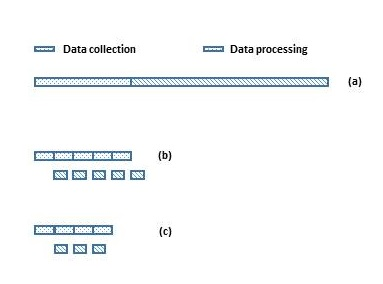
\includegraphics[width=0.65\linewidth]{../figure/pipeline} \\
\caption{\label{fig:pipeline} The benefit of pipelined authentication: (a) shows the original latency to collect and process a 10-second sample (numbers taken from Figure~\ref{tab:glass}, (b) shows the much reduced latency by breaking the 10-second signal to five 2-second chunks and pipeline the collection and processing procedures, and (c) shows that the delay can be further reduced if using a portion of the signal can correctly infer the classification result.}
\end{wrapfigure}
In this project, we propose to address this challenge by adopting the well-known pipeling technique, which is motivated by the characteristics of~\systemname. Suppose the original signal duration is $T$, and we have $T=nt$ with $n$ being an integer and $t<2$ seconds. Let us assume that the processing delay is less than $t$ when the sample duration $t$ is less than 2 seconds.  Then we can explore the following pipelining method. In the first $t$-second window, the system collects the $ACC$ sample for $t$ seconds. In any subsequent $t$-second window, the system continues to collect the $ACC$ sample for $t$ seconds, and at the same time, processes the portion of the sample collected in the previous window. We refer to this method as \emph{pipelined authentication}.


The proposed pipelined authentication can reduce the overall authentication latency in several ways. First, we overlap data collection and data processing to reduce the overall delay. Second, since processing shorter samples incurs less (than linear) latencies, by breaking a sample into smaller chunks can reduce the total latency. For example, using the numbers presented in Figure~\ref{tab:glass}, we find that processing one 10-second sample takes much longer time than processing one 6-second, one 2-second, and two 1-second samples. Third, now we can conduct what we call ``early classification'' -- maybe using a portion of the sample can already reveal the classification result -- and then we don't need to collect/process the entire sample. That is, we can dynamically determine the shortest sample duration we need. Combing these factors, we can achieve much reduced authentication latency (i.e., shorter data collection and shorter processing delays). Figure~\ref{fig:pipeline} illustrates the benefit of the proposed pipelined authentication scheme.



\vspace{4pt}\textbf{Authentication with Fewer Samples:} Another optimization we will explore is authenticating users with fewer samples. We can attempt to reduce the number of samples in several ways. First, we can minimize the number of samples for the legitimate user in the training set. It is thus a tricky question to determine how many and which samples should be used. In this project, we will explore only using the ``representative'' samples -- i.e., those that are the most similar to the rest of the user's samples. In this way, the computation/energy consumption in the authentication session can be greatly reduced.

Another optimization technique we can adopt is to dynamically adjust the sampling rate in the test phase. A lower sampling rate leads to fewer data points in a sample, thus shorter collection and processing latencies. In this project, we will explore dynamically adjusting the sampling rate based upon the temperature of the device. Namely, if we notice the device is becoming heated, then we should reduce the sampling rate. In the project, we will carefully quantify the interaction between the device temperate and the sampling rate.


\section{Evaluation Plan}\label{sec:eval} \vspace{-6pt}
\subsection{Developing~\systemname~App on Google Glass and Moto 360}\label{subsec:app}
In this proposal, we propose a body-movement pattern based authentication system, ~\systemname, for
wearable devices. In addition to developing and evaluating the proposed algorithms, we will also conduct in-depth evaluation of the~\systemname~system design. Even though there are many types of body movements that we can exploit for authentication purposes, in this project we will focus on the movements that can be easily captured by Google Glass (representing smart glasses) and those by Moto 360 (representing smart watches). Specifically, we will study the following movement patterns:
\begin{wrapfigure}{r}{3.0in}\centering
\begin{tabular}{cc}
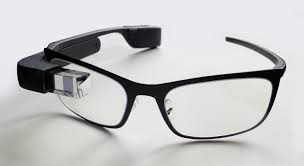
\includegraphics[width=0.45\linewidth]{../figure/glass1.jpg} &
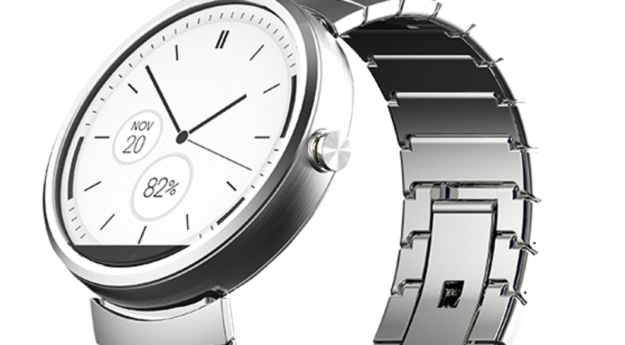
\includegraphics[width=0.45\linewidth]{../figure/moto} \\
(a) & (b) \\
\end{tabular}
    \caption{\label{fig:devices} We will implement~\systemname~on (a) Google Glass and (b) Moto 360 smart watch.}
\vspace{-6pt}
\end{wrapfigure}
\begin{itemize}
\vspace{-2pt}\item \emph{Movement patterns for smart glasses:} As far as smart glasses are concerned, we will explore head movement patterns (with music), eye blinking/winking patterns (with music), and pulses measured at the temple.

\vspace{-2pt}\item \emph{Movement patterns for smart watches:} As far as smart watches are concerned, we will explore arm movement patterns (with music), wrist movement patterns (with music), finger movements (with music), and pulses measured at the wrist.
\end{itemize}

We will choose easy-to-follow and fast-tempo music tracks (10 seconds long) as external stimuli. The readers can download such an audio track at our web site: \emph{http://www.winlab.rutgers.edu/~sugangli/somebody.midi}.

\subsection{Data Collection}\label{subsec:user}
\begin{wrapfigure}{r}{3.0in}\centering
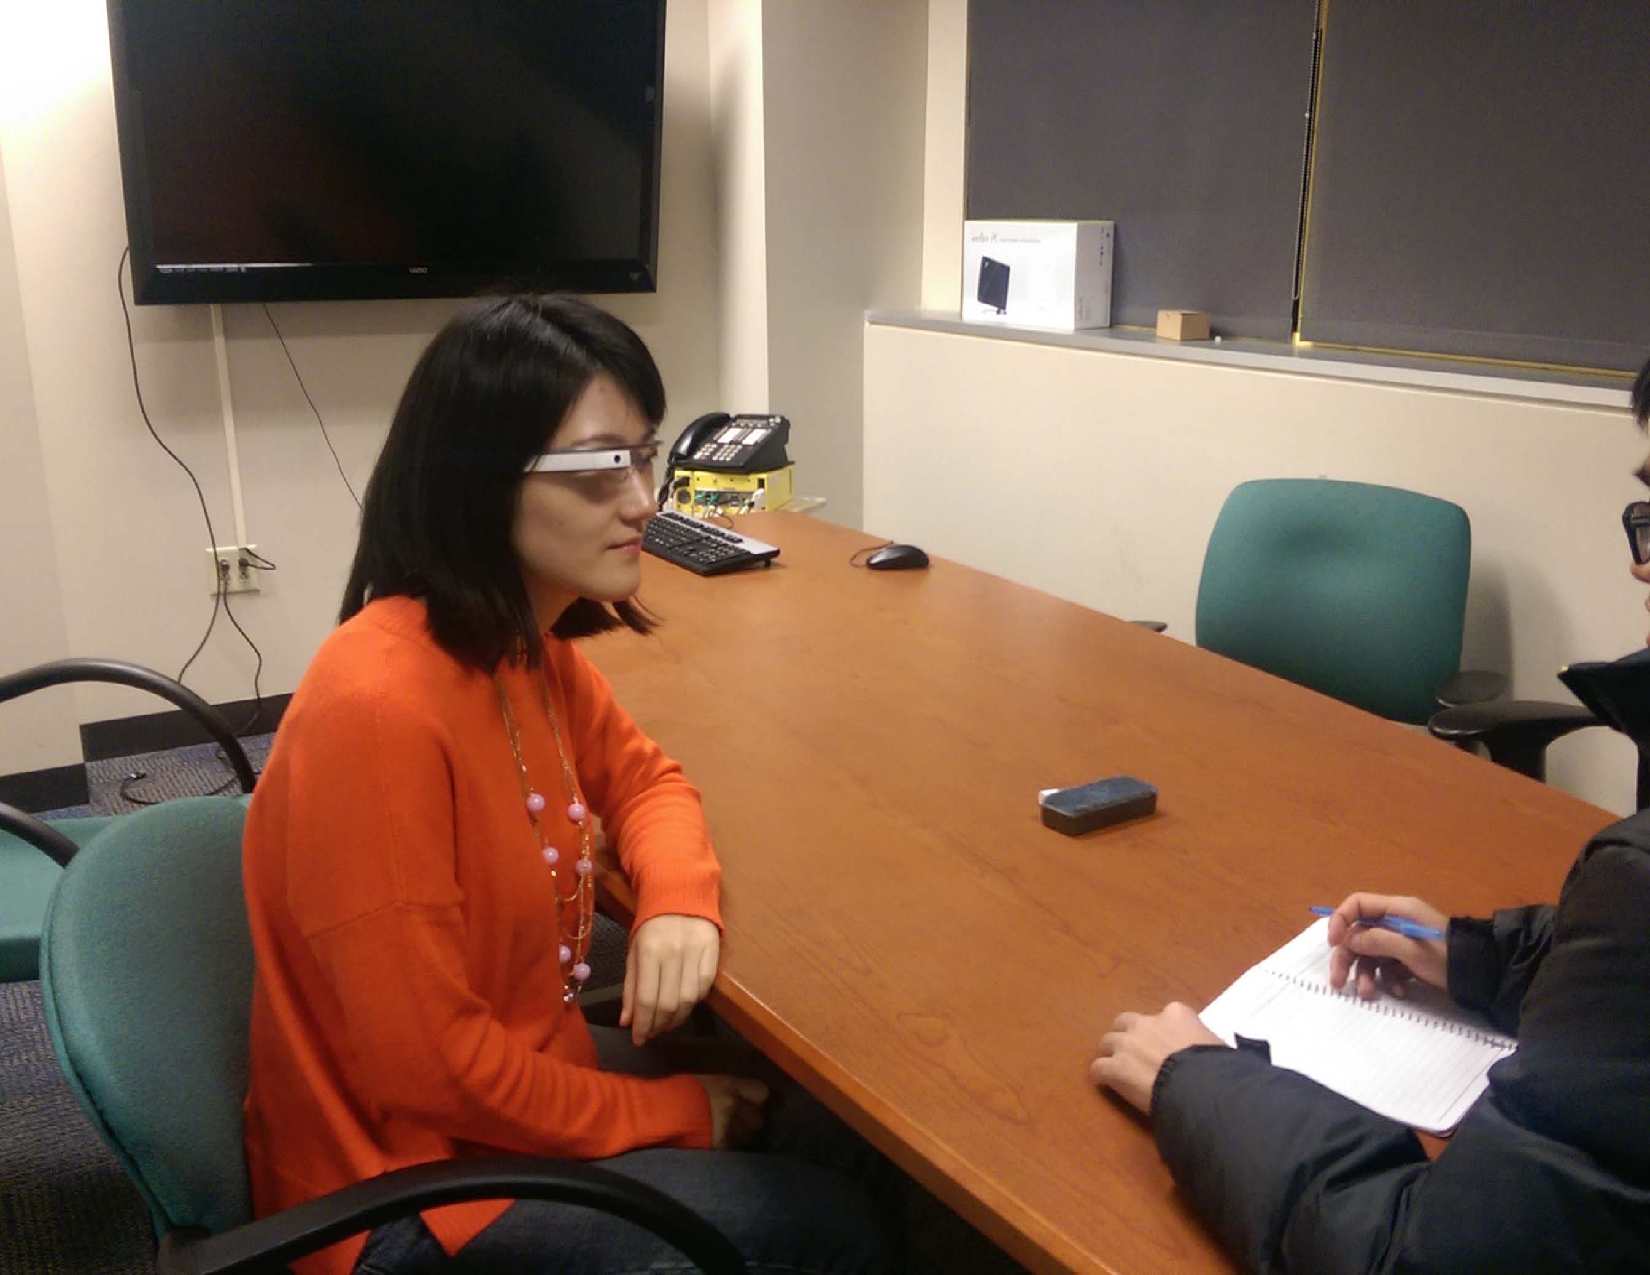
\includegraphics [width=.75\linewidth]{../mobisys_paper/fig/exp.pdf}
\caption{Our team member was collecting data with one of the participants in the preliminary study. \label{fig:exp}}
\end{wrapfigure}

The key to the success of this project is to collect data from a large and diverse set of participants, in different environments and contexts.  In this three-year project, we plan to collect data from 30 subjects. We will make effort to recruit participants such that we have a balanced mix of gender, age, height, and handedness. We plan to pay each subject \$15 for their particpation.

In the data collection session, we will inform the participants of the potential risks involved in wearing Google Glass and collecting head-movement or eye blinking/winking/pulse data (e.g., feeling dizzy after head-movement for a period of time, not being able to see clearly if near-sighted, etc.), as well as the potential risks in wearing Moto 360 and collecting hand-movements/pulse data (e.g., wrist pain). If they agree to participate, we will ask each subject to report their age and gender. We will help the subjects to wear the Google Glass and make head movements and eye blinking/winking while listening to the music track of their choice. We will also help the subjects to wear the Moto 360 and make wrist/hand movements while listening to the music track of their choice. Meanwhile, we will record the raw accelerometer data, raw gyroscope data, and the infra-red sensor data from the Google Glass.  Each recording session will be 10 seconds long, and we (the graduate students) will sit through each session with the subject to help him/her use the system properly, as shown in Figure~\ref{fig:exp}. After every 5 recording sessions, we will ask the subject to take a break to relax their muscle and regain energy. We will also split each subject's data collection session on different days, to include natural movement variability in the data sets. 


\subsection{Long Term App Deployment and  Evaluation} After evaluating and revising the app design using realistic user data, we will install the~\systemname~app on five Google Glasses and five Moto 360 watches. We will ask ten participants to use these devices on a daily basis for three months. During the evaluation period, each participant is the legitimate user of the device, and they will invite friends and family members to try to log in to the device from time to time. The authentication records will be logged and synced to the cloud, which we will monitor remotely. After the evaluation period, we will carefully study the authentication logs, find the flaws (if any) in our design and improve the design if necessary. 

\begin{figure}[t]
\centering
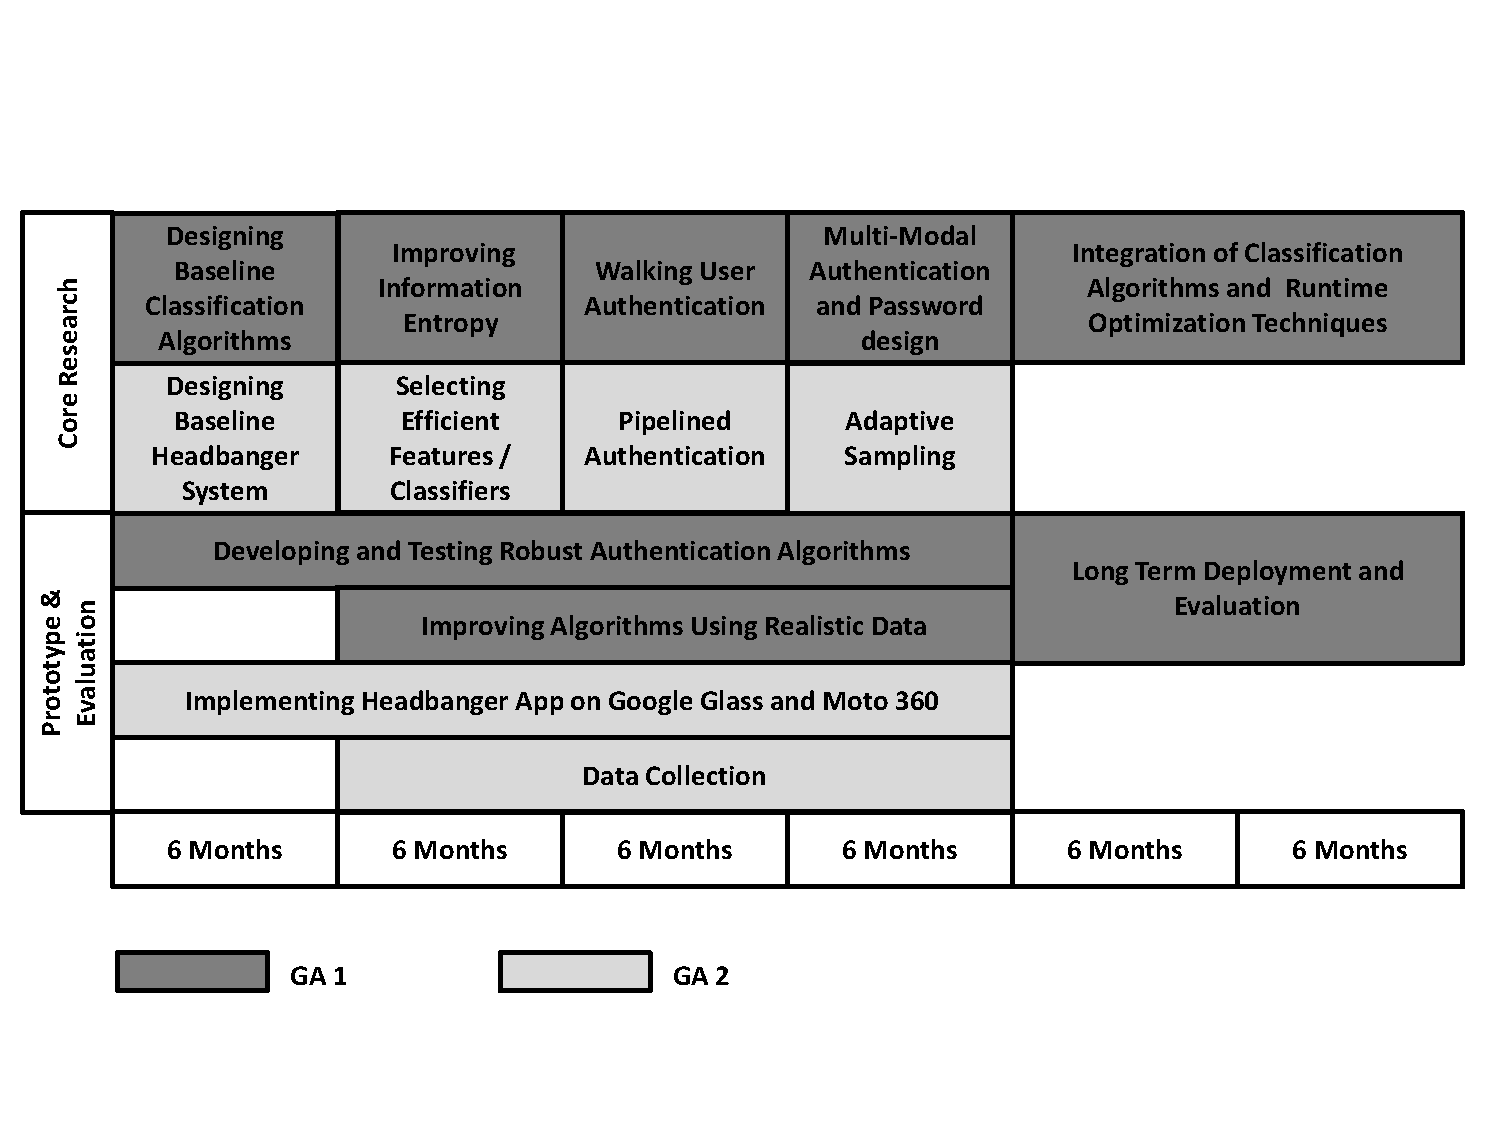
\includegraphics[width=.5\columnwidth]{../figure/plan.pdf}

\vspace{-12pt}\caption{\label{fig:plan}The detailed 3-year work plan.} \vspace{-12pt}
\end{figure}

\subsection{Work Plan}\label{subsec:plan}\vspace{-6pt}
This proposed project is a collaborative research between two PIs from Winlab, Rutgers University, where Prof. Zhang's research focus is on sensing and mobile computing, while Prof. Gruteser's research focus is on mobile computing, security and privacy. In addition to the two PIs, we have budgeted for 2 GAs in the first two years, and 1 GA in the third year. The detailed work plan is summarized in Figure~\ref{fig:plan}.
\vspace{-6pt}
\section{Curriculum Development Activities and Broader Impact}\label{sec:education}\vspace{-6pt}

The proposed research consists of an important curriculum development effort. The PIs are planning to create a graduate level seminar course, entitled ``Security and Privacy Issues for Wearable Computing,'' with a special focus on issues such as data security and privacy, user authentication, and ultra low-power security for wearable devices. Students will read recent papers from leading conferences or journals in related fields such as ACM CCS, IEEE Symposium on Security and Privacy, Usenix Security, ACM Mobisys, IEEE Transactions on Mobile Computing, etc. The reading list will include enabling wearable technologies, their security and privacy concerns, as well as emerging applications for wearable devices. For this course, students will collaboratively work on research-oriented open-ended projects that focus on designing and evaluating security/privacy preserving algorithms for emerging wearable devices and applications.


%\section{Broader Impact}\vspace{-6pt}
%The proposed project has a broad and profound impact on many aspects of society, and can contribute to the achievement of societally relevant outcomes.

\vspace{6pt}\noindent\textbf{Preparing the next-generation workforce for a rapidly growing industry.} Smart sensors and wearable devices are predicted to be the next computing platform that will seamlessly weave into our everyday life. In fact, a large number of startups are emerging in the general areas of wearable technology~\cite{nymi,scheirer1999expression,di2005magic,choudhury2002sociometer,meyerhoff1993line,starner2000gesture,farringdon1999wearable,led2004design,hung2004wearable,mistry2009sixthsense,giansanti2008assessment}. To respond to this trend, it is important to thoroughly understand its impacts on people's security and privacy, and to be equipped with technologies to address these concerns. The proposed research and education activities will play the critical role of preparing the next-generation workforce in this promising and rapidly growing area.

\vspace{3pt}\noindent\textbf{Engaging Undergraduates and the Youth in Research:} As part of the broader impacts, the PIs plan to involve undergraduate students and talented students from local high-schools. Prof. Zhang has served as the faculty advisor for the Eta Kappa
Nu honor society for over 5 years. She has already worked with four undergraduate students from the honors program on related research projects, with publications coming out of several of these efforts (e.g.~\cite{jsspp03,sensorfusion05,xu:wise04,xu:mobihoc05}).

The PIs will also actively engage high school students through summer research experiences in this project. In particular, the team will accept students from the Liberty Science Center's Partners in Science program and the WINLAB summer research program. Third, the Rutgers team plans to accept an academic year intern from Bergen County Academies, a NJ magnet school that operates an intern program for its high school students and to identify appropriate independent study topics that allow undergraduate students to participate during the academic year. PI Gruteser will draw from his established relationships with these programs and his past mentees include students that have won prizes at regional high school science competitions and started undergraduate computer science programs at UC Berkeley and Stanford. Additionally, Prof. Zhang has been engaged in an outreach to local high school students (Highland Park and Franklin High Schools in NJ).

Moving forward, the team will continue to develop undergraduate research projects, offer summer internships to undergraduate and high school students, and encourage them to work in related fields.


\vspace{3pt}\noindent\textbf{Encouraging Female Students in Engineering:} Ensuring that Science, Technology, Engineering and Mathematics (STEM) reaches as broad of a base as possible is an important activity that the investigators intend to focus on.
Professor Zhang has been actively involved in The Society of Women Engineers at Rutgers
University, where a series of workshops and luncheon meetings are
organized each semester, to give talks that emphasize the important
leadership roles open to women in EE/CS. She has supervised three female Ph.D. students, more than ten female master students and two female undergraduate students (both went to graduate school). One of her former Ph.D. students is now a tenured Associate Professor at University of South Carolina.  In addition, she has
organized a panel that discussed the challenges a woman engineer may
encounter in her career, which was very well received among woman
engineering students. Prof. Gruteser has also advised four additional female PhD students and a recent female high school student mentee has just been accepted to Princeton University’s undergraduate computer science program. Moving forward, the PIs will continue their effort to encourage female students to engage in STEM.
\vspace{-8pt}

%\input{WellMon_perspective}
\section{Results from Prior NSF Projects}\label{sec:prior}\vspace{-8pt}

\noindent \textbf{Y. Zhang} has, in the last 5 years, been the PI on NSF grants:
(i) CNS-0546072,  ``CAREER:PROSE: Providing Robustness in Systems of Embedded Sensors'', \$484K,  7/1/06 - 6/30/11;
(ii) CNS-0831186, ``CT - ISG: ROME: Robust Measurement in Sensor Networks'', \$400K, 09/01/08-08/31/11;
and co-PI on NSF grants
(iii) CNS-0910557, ``TC:Large: Collaborative Research: AUSTIN-- An Initiative to Assure Software Radios have Trusted Interactions'', \$410K, 9/1/09 - 8/31/12, (iv) CNS-1040735, ``FIA: Collaborative Research: MobilityFirst: A Robust and Trustworthy Mobility-Centric Architecture for the Future Internet'', \$2.73M, 9/1/10 - 8/31/13, and (v) CNS-1423020, ``NeTS: Small: Transmit Only: Cloud Enabled Green Communication for
Dense Wireless Systems'', \$4.98M, 9/1/14 - 8/31/17.
The \emph{intellectual merit} from these research projects have led to several new contributions in the past 5 years to the areas of sensing and Internet of things~\cite{zan-etal:mdm10,sun2012association,sun2011improved,sun2012boomerang,moore2013building}, unobtrusive human context learning ~\cite{xu2012improving,xu2012towards,xu2013crowd++,xu2013scpl}, network virtualization~\cite{bhanage2011virtual,bhanage2011experimental}, and next generation Internet architecture design~\cite{vu2012dmap,sun2011improving,zhang2012content,liu2013secure,zhang2013using,li2013mobile,li2012popularity}. \emph{Broader Impact}: Dr. Zhang has advised 7 Ph.D. students,  has created Owl Platform (www.owlplatform.com), a low-power smart home sensing system based on results from prior NSF grants, has developed the global name resolution service prototype for the GENI national testbed, has redesigned the Computer Architecture, Database Systems, and Performance Evaluation courses at Rutgers-ECE. She is currently working with four Ph.D. students.

\textbf{Marco Gruteser} is an Associate Professor at WINLAB Marco Gruteser and has served as PI and Co-PI on several NSF projects in the areas of networking, vehicular applications, and privacy. As PI for a location privacy
project~\cite{nsf-ct-anonymity} he has also developed the path cloaking methods for
protecting privacy of time-series location traces~\cite{1315266_hoh_privacy_gps,
hoh06:_enhan_privac_preser_anony_locat} as well as the virtual trip line privacy
mechanisms and a corresponding secret-splitting architecture for protecting
privacy in probe vehicle-based automotive traffic monitoring
systems~\cite{hoh_virtual_trip_lines,1717364_hoh_privacy_traffic_monitoring}.
All together, ten PhD students have to date completed their degrees and the projects lead to deep industry collaborations with General Motors, NEC Labs, as well as product
development impact at Nokia with privacy technologies, and outreach to the general public by featuring into online, radio, and television media (e.g., MIT Technology Review, NPR, and CNN TV).

\newpage

\setcounter{page}{1}
\def\mysection{D}
\bibliographystyle{plain}
\bibliography{../mobisys_paper/sugang,yyzhang,MG_prior}
%\bibliography{../elder,../chenren,../audio,../yyzhang,../education,../ben,../lin,../system,../RefsForYanyong,../janneown,../nsf-hui,../WadeEAMonRefs,../hui1}

\end{document}
